\documentclass{article}

\usepackage{cmcphys}
\usepackage[margin=1.0in]{geometry}
\usepackage[titletoc,title]{appendix}
\allowdisplaybreaks

\graphicspath{{figures/}}

\renewcommand{\figurename}{Fig.}
\renewcommand{\L}{\mathcal{L}}
\newcommand{\e}{\mathrm{e}}
\renewcommand{\i}{\mathrm{i}}
\renewcommand{\Re}{\mathrm{Re}\ }

\title{Chaotic Behavior of the Triple Pendulum \\
    \large A Computational Approach }
\author{Rachel Bass \and Cory McCartan}
\date{May 2017}

\begin{document}

\maketitle

\begin{wrapfigure}[16]{R}{0.2\textwidth}
	\centering
	\includegraphics[width=0.17\textwidth]{drawing.tikz}
    \caption{The triple pendulum.} 
    \label{fig:pendulum}
\end{wrapfigure}

\section{Introduction}
The triple pendulum is a classic example of a mechanical system that can be
described simply yet behaves chaotically under a wide variety of initial
conditions. Compared to the double pendulum, the addition of another mass (and
accompanying coordinate $\phi_3$) adds significantly more complexity and
non-linearity to the system dynamics. We study the conditions under which the
triple pendulum is chaotic for the special case of equal lengths and masses of
the pendula (see Fig. \ref{fig:pendulum}). We identify several critical
values for initial conditions, beyond which the pendulum generally behaves in a
chaotic manner.

\section{Modeling}
Before we model the triple pendulum, we need to find the system's 
equations of motion.  The Lagrangian of the system is
\begin{align}
    \L &=  mgl\left(3\cos\phi_1+2\cos\phi_2+\cos\phi_3 \right) 
	   + \frac{1}{2}ml^2 \bigl( 3\dot\phi_1^2+2\dot\phi_2^2+\dot\phi_3^2 \\
	   &\qquad\qquad + 4\dot\phi_1\dot\phi_2\cos(\phi_1-\phi_2)   
	   + 2\dot\phi_1\dot\phi_3\cos(\phi_1-\phi_3)
	   + 2\dot\phi_2\dot\phi_3\cos(\phi_2-\phi_3) \bigr). 
\end{align}
For more details, see Appendix A. 
We make the simplifying assumptions that all three masses
are equal, and that the connecting rods are massless and of equal length.
From the Lagrangian, we find our equations of motion for the three masses. 
These equations are most easily expressed as a matrix equation:
\begingroup 
\begin{equation} \renewcommand*{\arraystretch}{1.25} 
	\resizebox{0.95\textwidth}{!}{$
	\begin{pmatrix}
		\ddot\phi_1 \\
		\ddot\phi_2 \\
		\ddot\phi_3
	\end{pmatrix} =
	\begin{pmatrix}
		3                    & 2\cos(\phi_1-\phi_2) & \cos(\phi_1-\phi_3) \\
		2\cos(\phi_1-\phi_2) & 2                    & \cos(\phi_2-\phi_3) \\
		\cos(\phi_1-\phi_3)  & \cos(\phi_2-\phi_3)  & 1                   \\
	\end{pmatrix}^{-1}
	\begin{pmatrix}
		-\dot\phi_3^2\sin(\phi_1-\phi_3) -2\dot\phi_2^2\sin(\phi_1-\phi_2)
			-\frac{3g}{l}\sin\phi_1 \\
		-\dot\phi_3^2\sin(\phi_2-\phi_3) + 2\dot\phi_1^2\sin(\phi_1-\phi_2)
			-\frac{2g}{l}\sin\phi_2 \\
		\dot\phi_2^2\sin(\phi_2-\phi_3) + \dot\phi_1^2\sin(\phi_1-\phi_3)
			-\frac{g}{l}\sin\phi_3
	\end{pmatrix}
	$} 
\end{equation} 
\endgroup 
Note that this matrix equation includes a matrix inverse. Instead of 
performing this tedious calculation by hand, we take advantage of the 
Python library \texttt{numpy} to perform the calculation. 

\section{Validation}

\begin{wrapfigure}[10]{R}{0.5\textwidth}
	\centering
	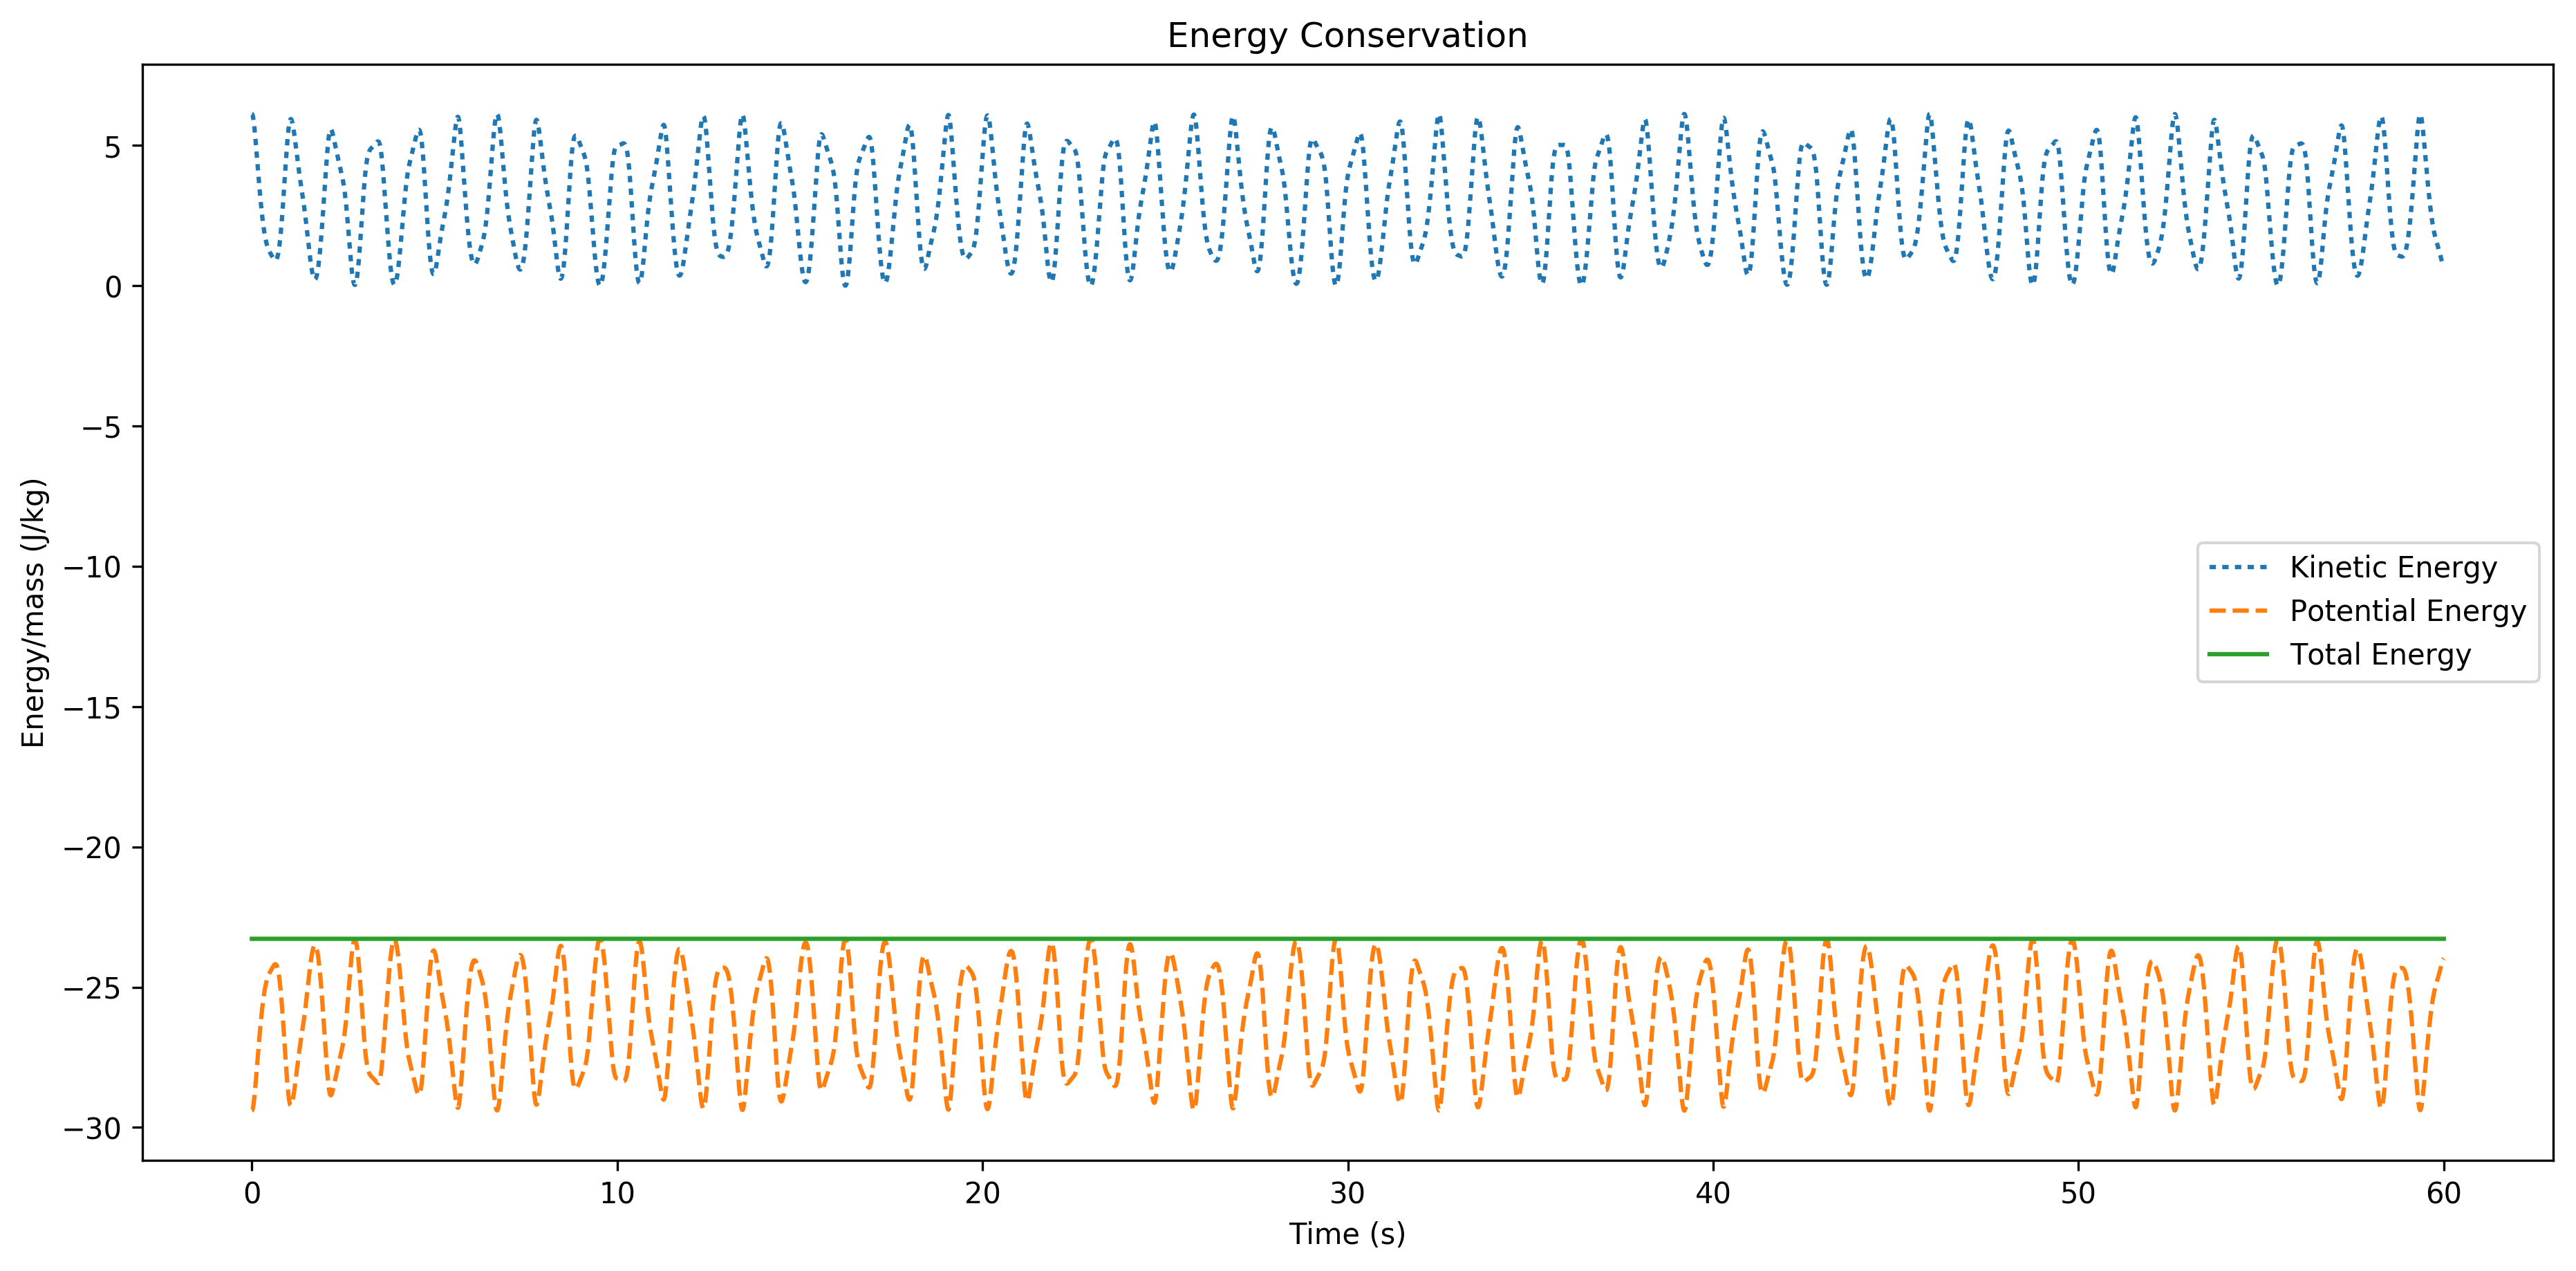
\includegraphics[width=0.5\textwidth]{energy_conservation}
	\caption{Kinetic, potential, and total energy over time for $\dot\phi_3(0)=\SI{7}{s^{-1}}$.}
	\label{fig:energy_cons}
\end{wrapfigure}

There is no analytical solution to above equations of motion.  The best 
way to verify our numerical solution is to check that energy is conserved.
Manually calculating the kinetic and potential energy from the numerical 
solution for the case with moderate initial angular velocity, we confirm 
that total energy is indeed conserved (Fig. \ref{fig:energy_cons}).

We also confirmed that with no initial angular velocity or displacement, 
the pendulum system remained motionless.

\section{Analysis}

\subsection{Fourier Transform}
Given the complexity of the system, it can be difficult to determine whether 
a given solution is periodic or not by merely looking at its time plot 
(Fig. \ref{fig:moderate_time}) or  phase space plot (the fact that the phase 
space is six-dimensional compounds these difficulties).  

\begin{figure}[ht]
	\centering
	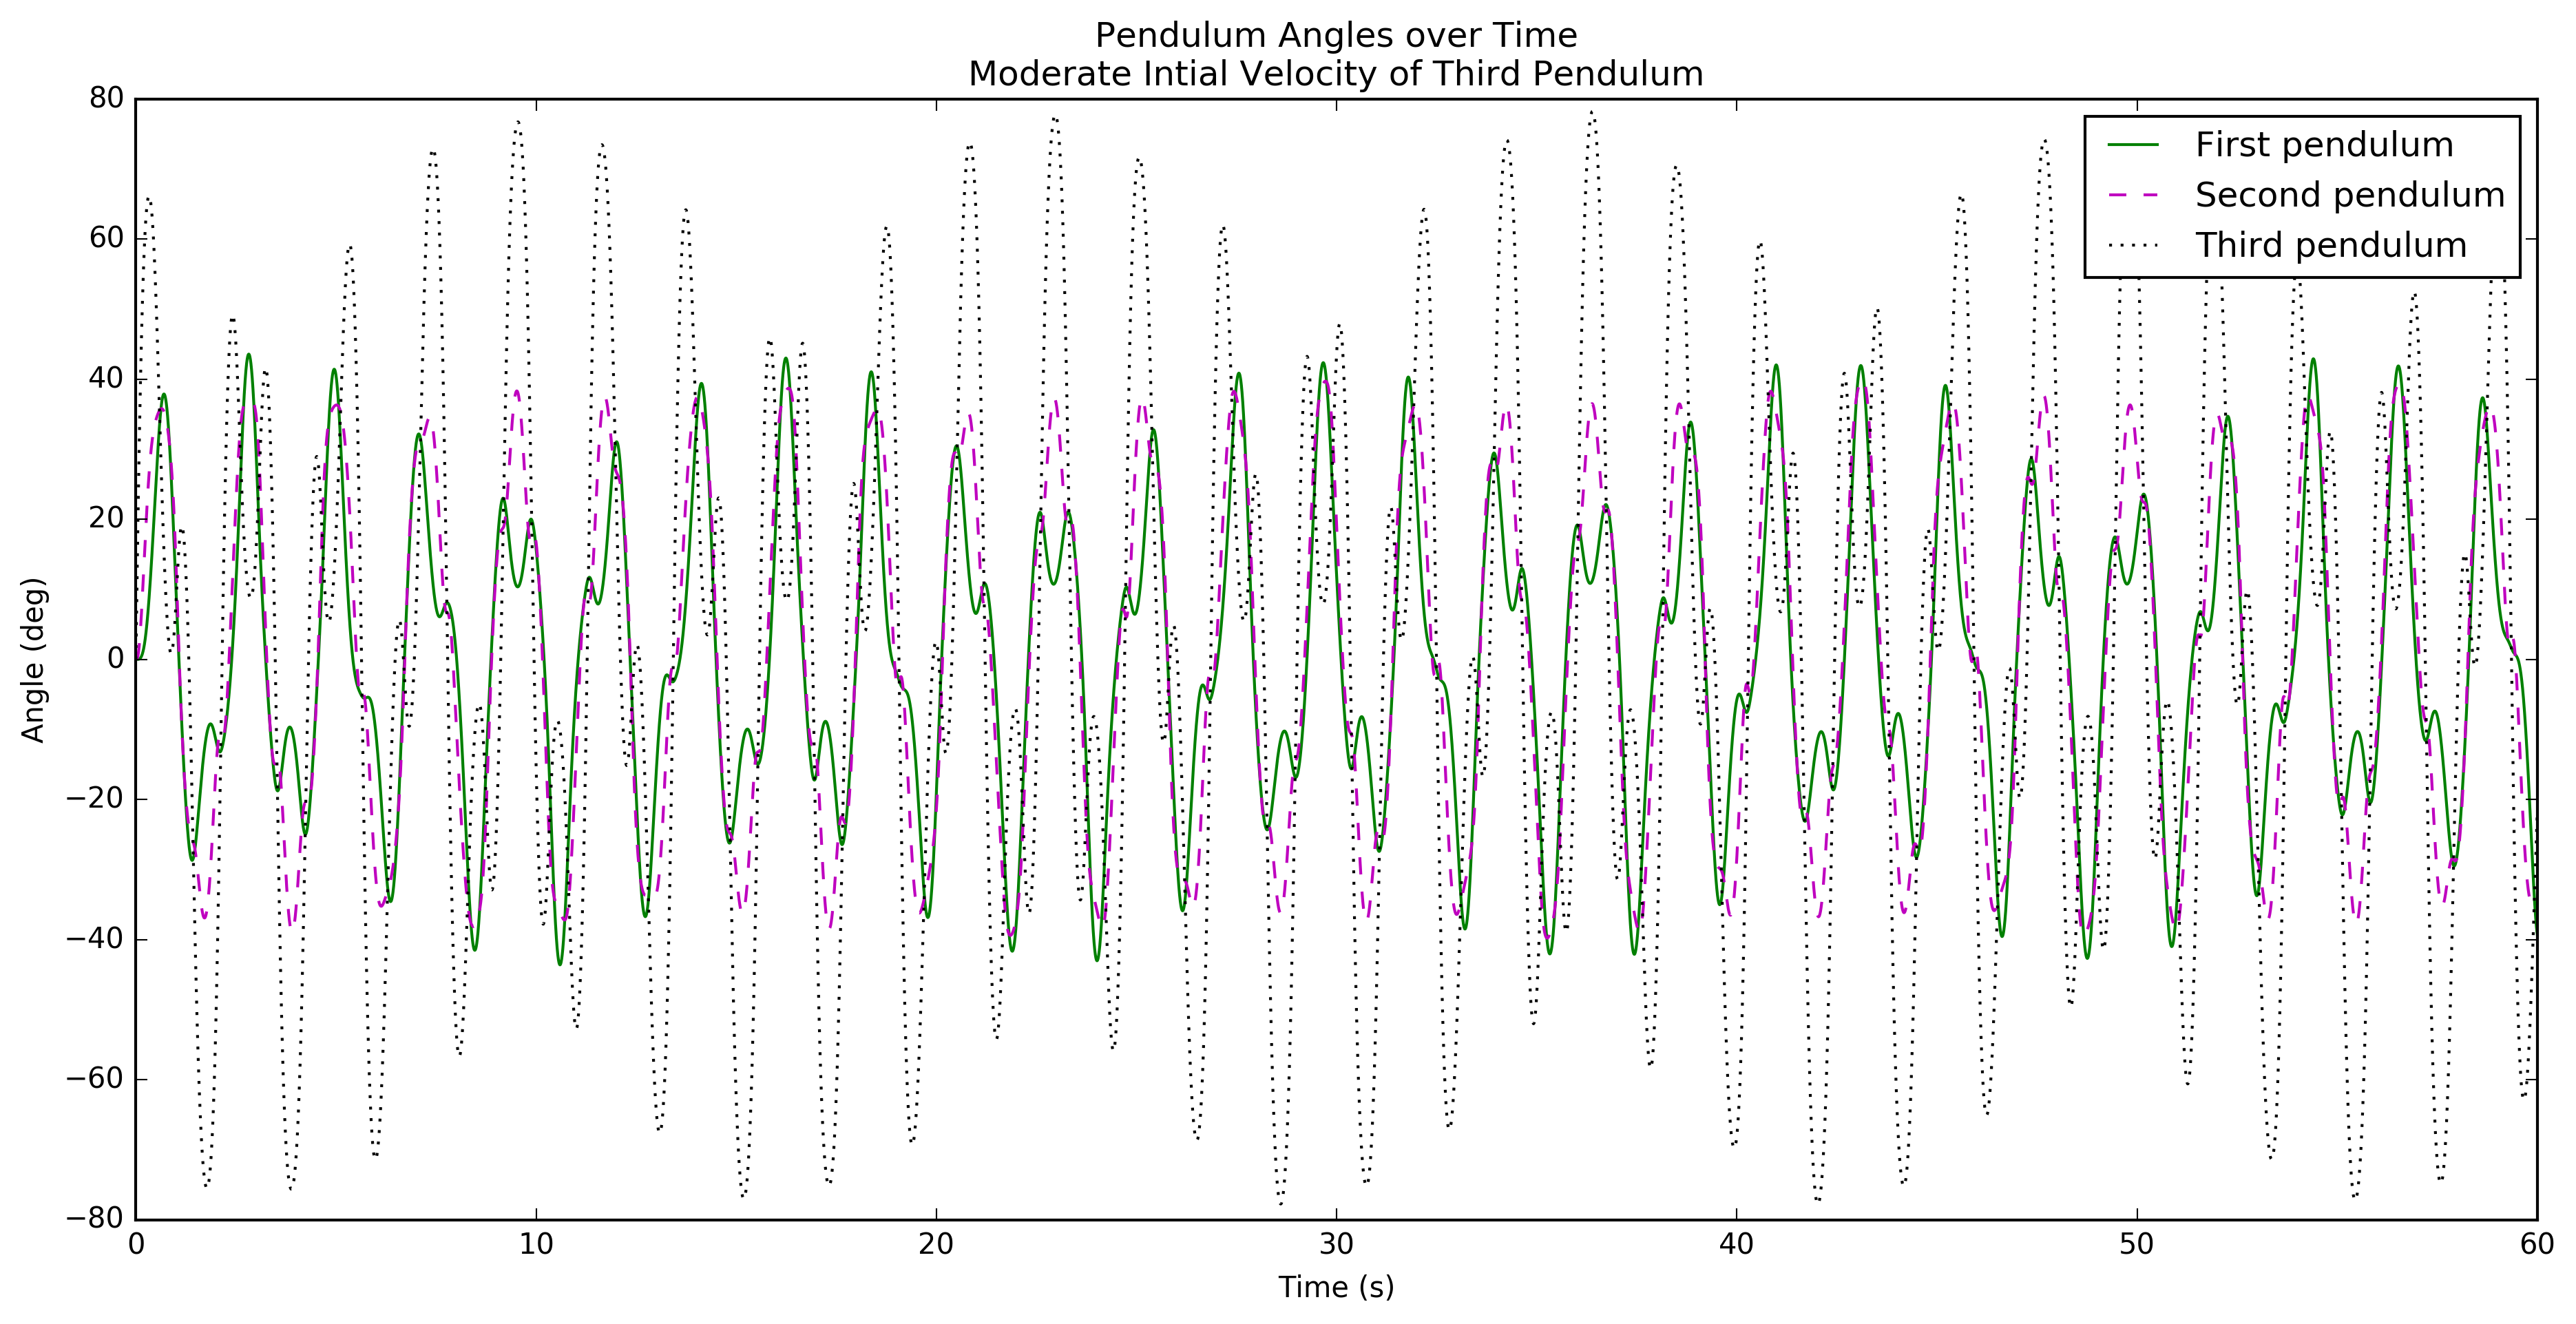
\includegraphics[width=0.8\textwidth]{moderate_velocity_time_sol}
	\caption{$\phi_1,\phi_2$, and $\phi_3$ over time for 
	$\dot\phi_3(0)=\SI{7}{s^{-1}}$.}
	\label{fig:moderate_time}
\end{figure}

A robust way to determine periodicity is to use the Fourier transform of the 
angle data. Periodic solutions have strong peaks at nonzero frequency values,
while chaotic solutions have no peaks other than a large singularity at zero 
(Fig. \ref{fig:fft}).

\begin{figure}[hbt]
    \centering
    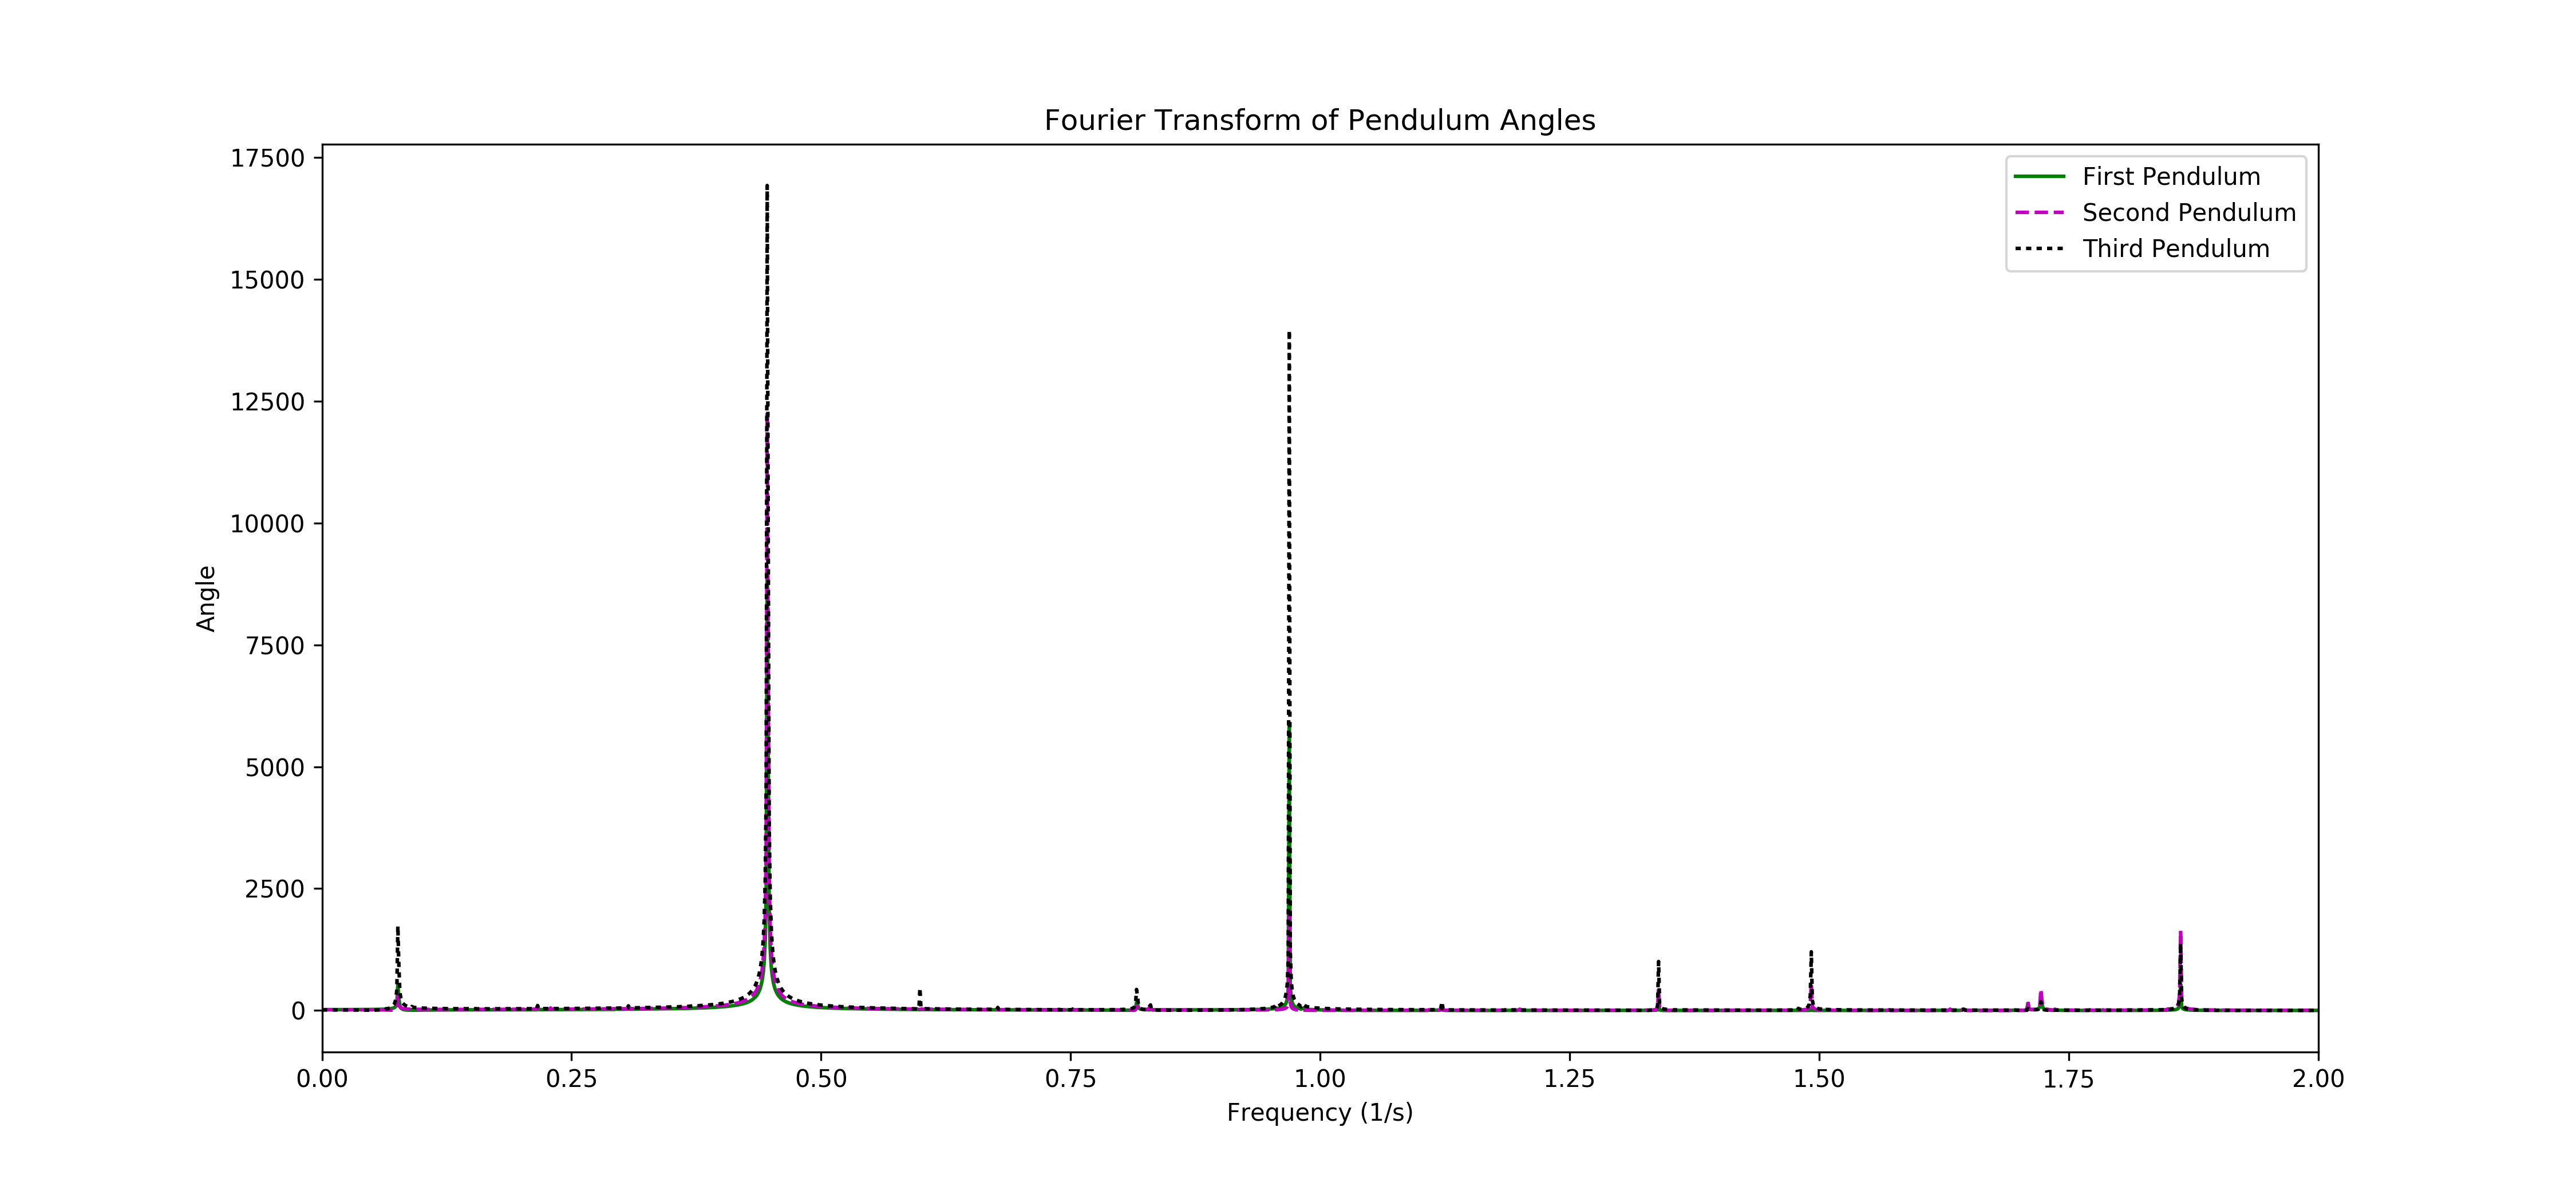
\includegraphics[width=0.49\textwidth]{fft_periodic}
    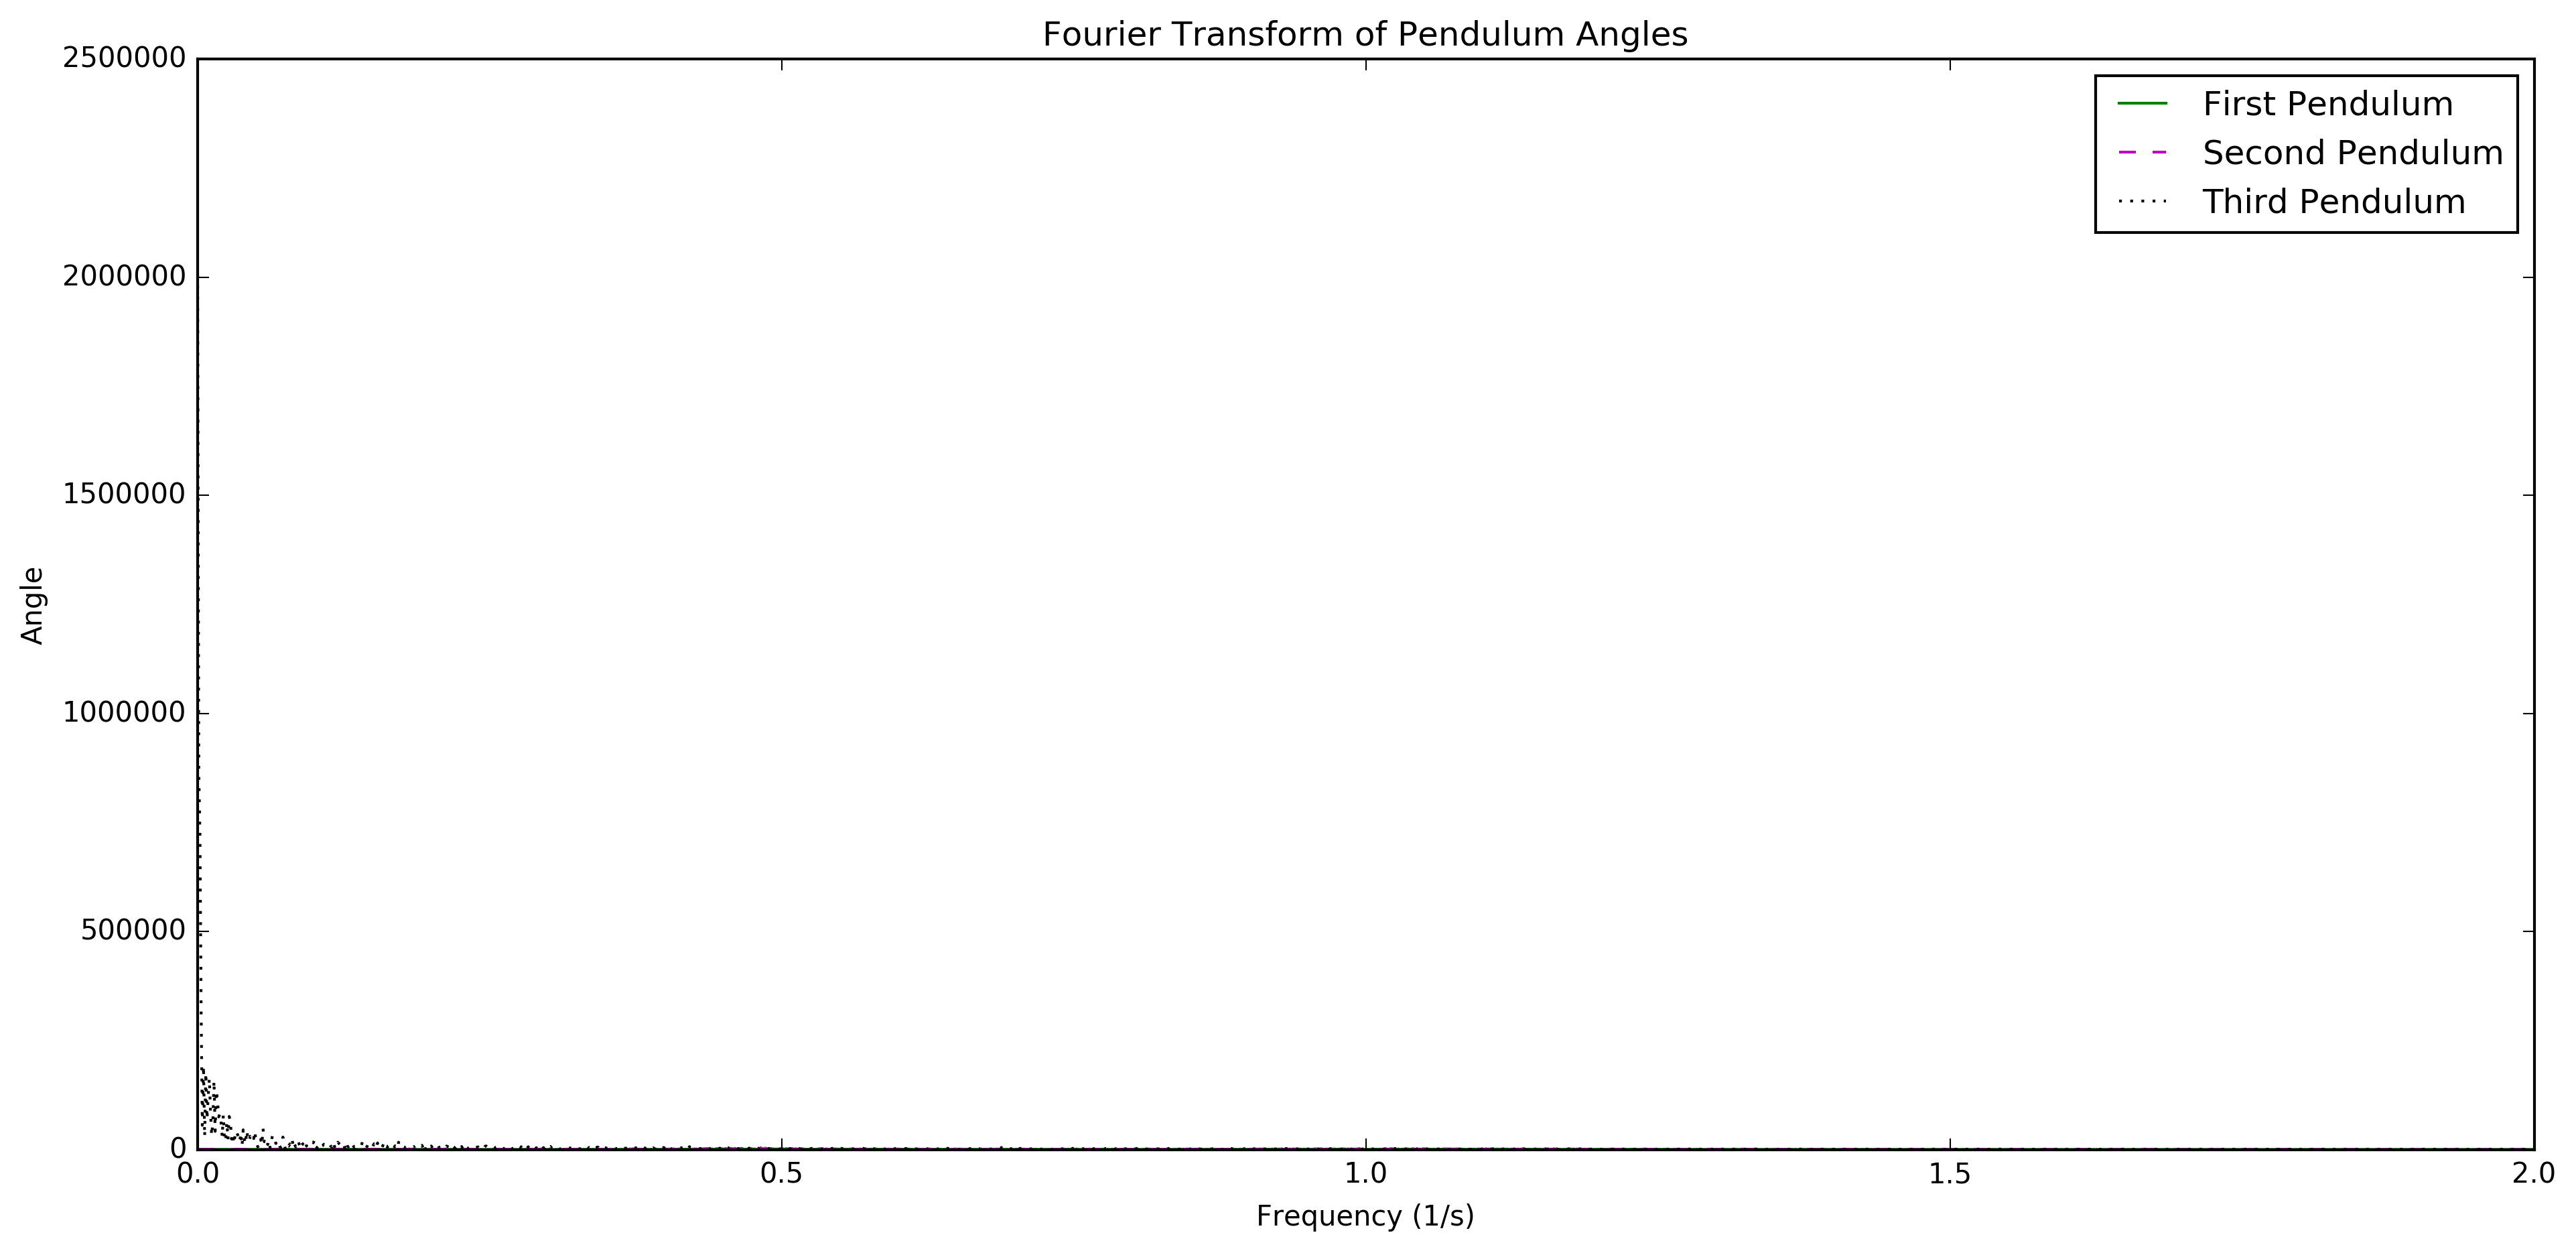
\includegraphics[width=0.49\textwidth]{fft_chaotic}
    \caption{The Fourier transform for $\phi_3(t)$.
        Left: $\dot\phi_3(0) = \SI{7}{s^{-1}}$.
        Right: $\dot\phi_3(0) = \SI{15}{s^{-1}}$. }
    \label{fig:fft}
\end{figure}

\subsection{Bifurcation Diagrams and FFT Contour Plots}
In chaotic systems such as the damped driven pendulum, there is a natural
frequency to the system, namely, the driving frequency. One can then sample 
the solution at time steps corresponding to this frequency to produce a
bifurcation diagram.  Unfortunately, there is no such natural frequency for
the triple pendulum system, which makes a traditional bifurcation diagram 
impossible.  We can, however, create a plot that can convey similar 
information. As in the bifurcation diagram, we simulate the system across 
a range of initial conditions. We take the Fast Fourier Transform (FFT) of 
each solution, and plot this as a column of pixels, where the logarithm of 
the Fourier transform is mapped to a color (magenta for low intensity, yellow 
for high intensity). 
\begin{figure}[h]
	\centering
	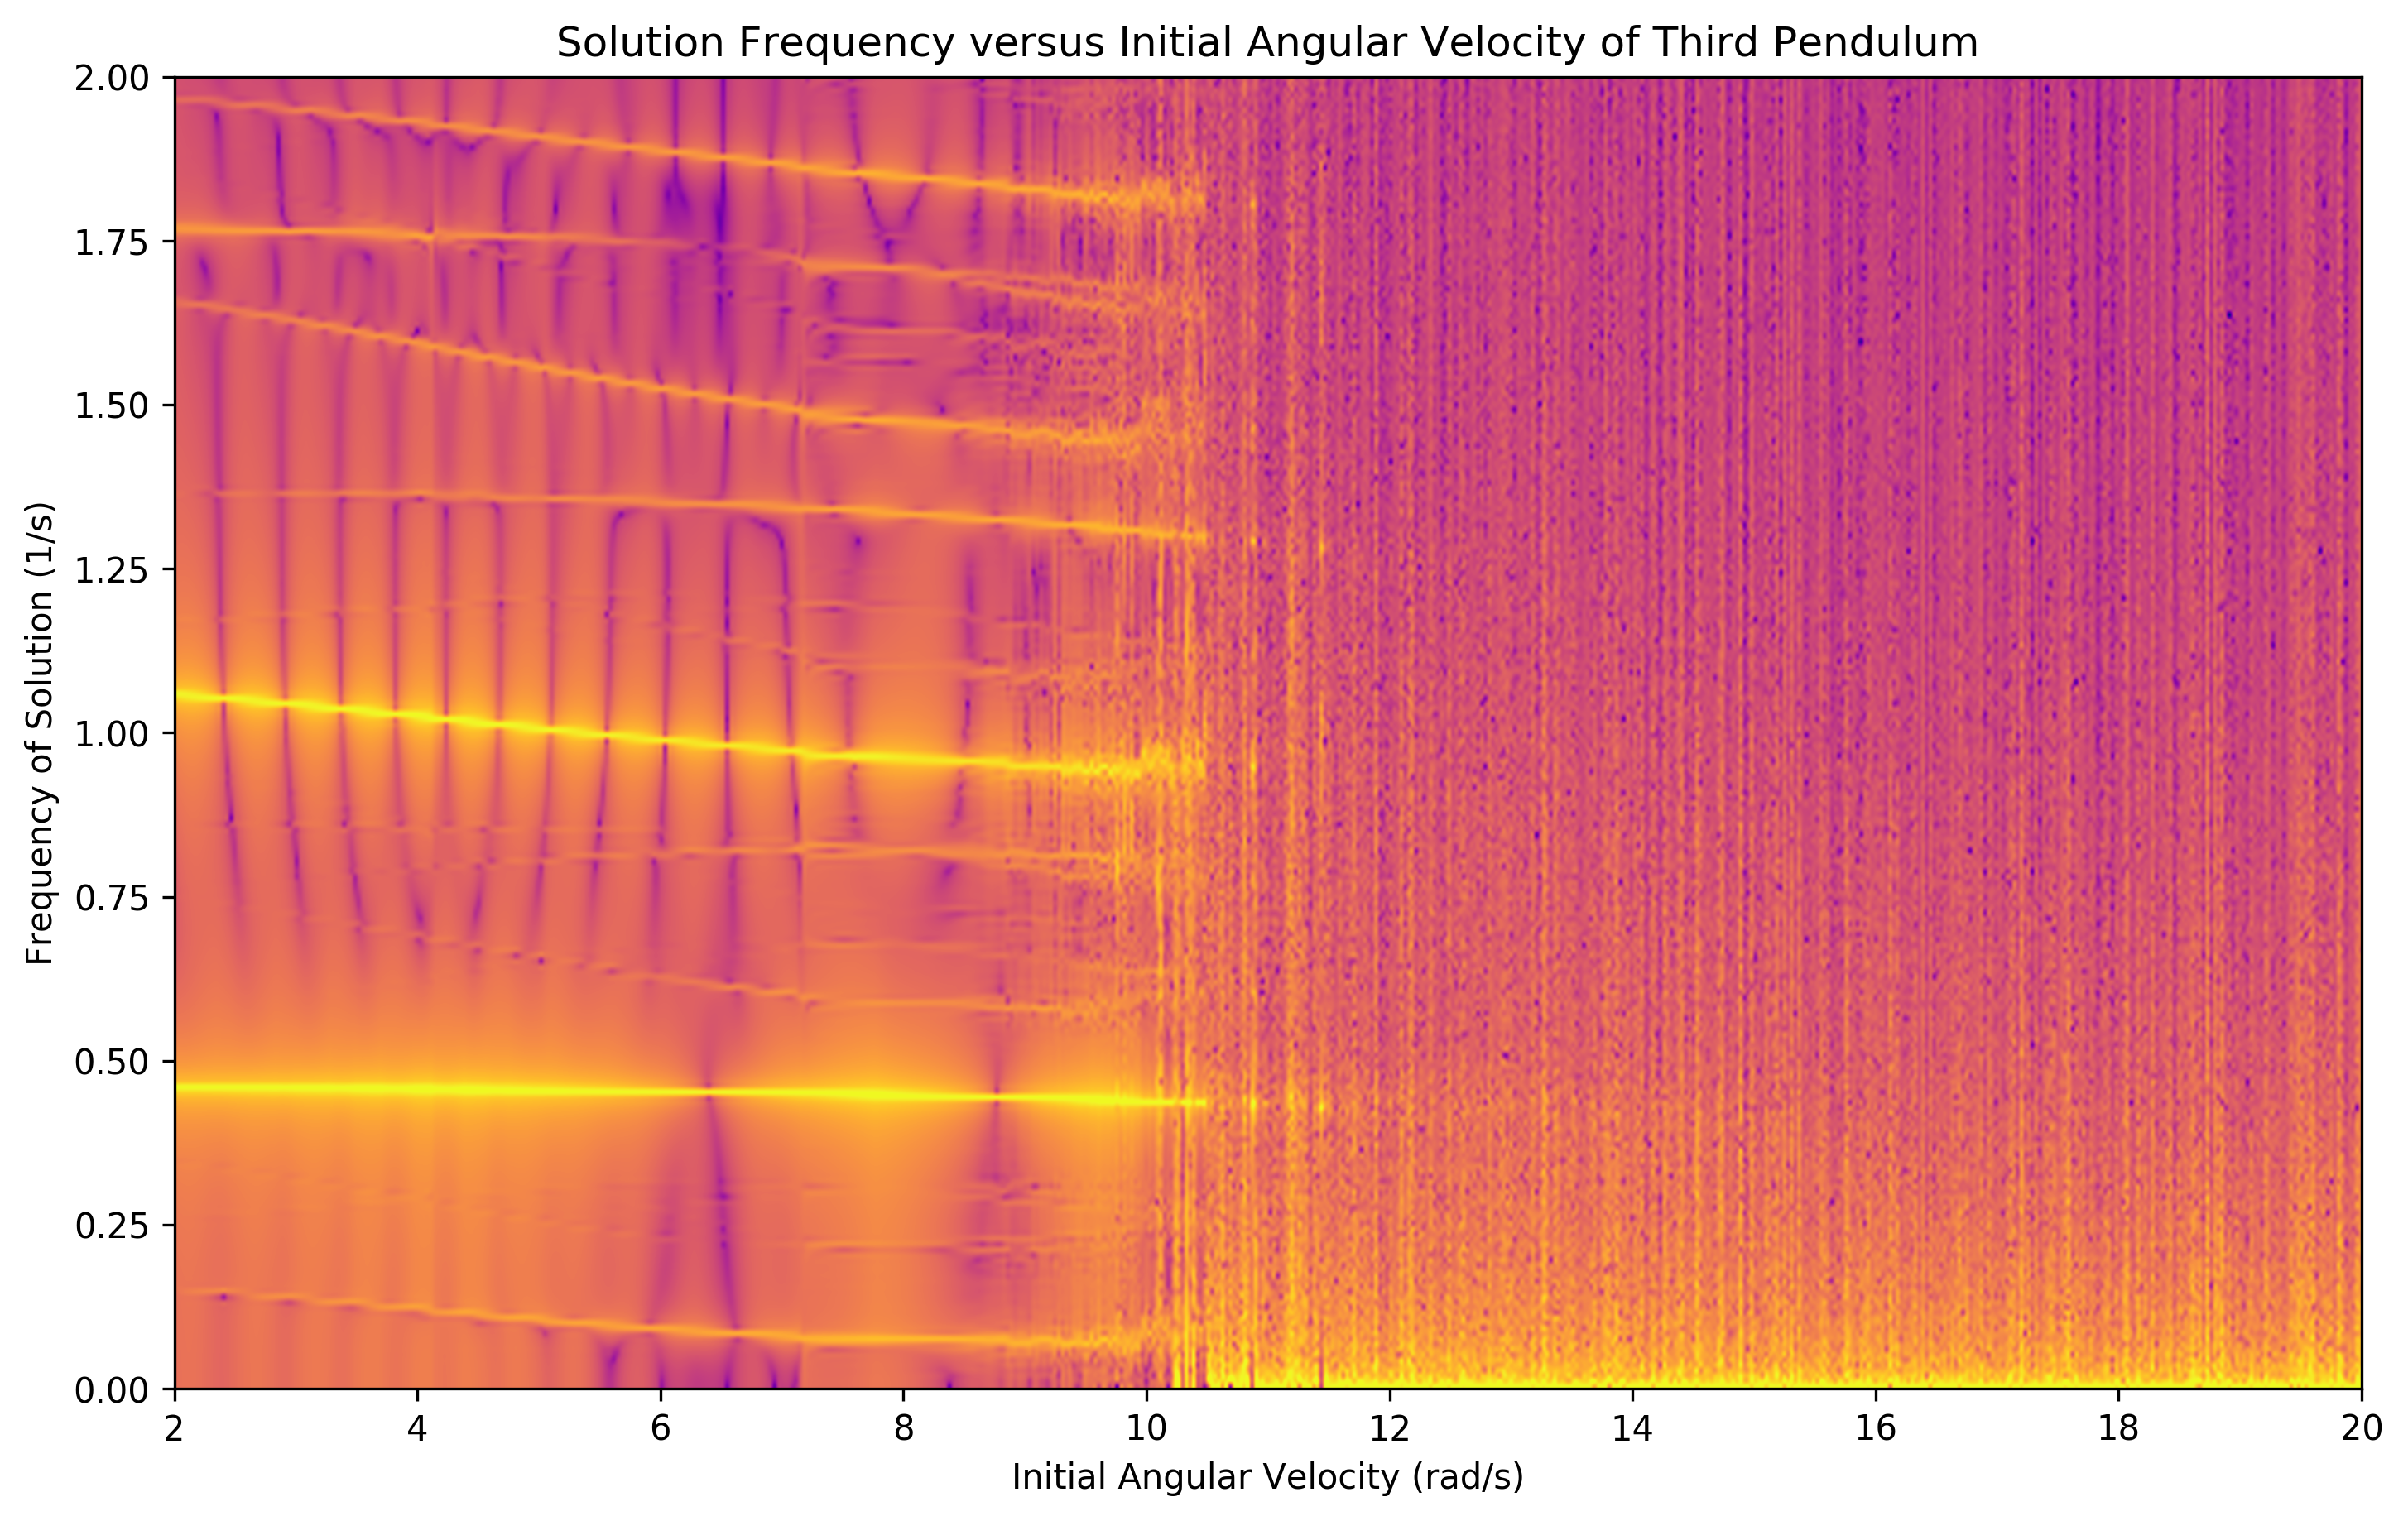
\includegraphics[width=\textwidth]{contour_3}
	\caption{FFT contour plot for $\SI{2}{s^{-1}}\le\dot\phi_3(0)
    	\le\SI{20}{s^{-1}}$.}
	\label{fig:contour_3}
\end{figure}
This allows us to see how the frequency composition of the
solution changes as an initial parameter is changed---and, importantly, when 
chaos sets in. We call this plot an FFT contour plot. Fig. \ref{fig:contour_3} 
shows the FFT contour plot for $\phi_3$ as $\dot\phi_3(0)$ is varied. We can
clearly see the two main frequency components from Fig. \ref{fig:fft} for 
low values of $\dot\phi_3(0)$, but these abruptly disappear around $\dot
\phi_3(0)=\SI{10.5}{s^{-1}}$. While there are short ``bursts" of periodicity
past this point, for the most part, chaos dominates.


\section{Results}

\subsection{Non-chaotic Behavior}
As seen in Fig. \ref{fig:contour_3}, the system is not chaotic for values of
$\dot\phi_3(0)\lesssim\SI{10.5}{s^{-1}}$. Fig. \ref{fig:moderate_time} shows 
the various angles over time, and Fig. \ref{fig:fft} shows on the left the 
Fourier transform of $\phi_3$. We can also change coordinates from $\phi_1,
\phi_2$, and $\phi_3$ to Cartesian coordinates, which allows us to plot
the actual trajectories the masses trace out over time (Fig. 
\ref{fig:moderate_trajectories}).

\begin{wrapfigure}[13]{r}{0.5\textwidth}
	\centering
	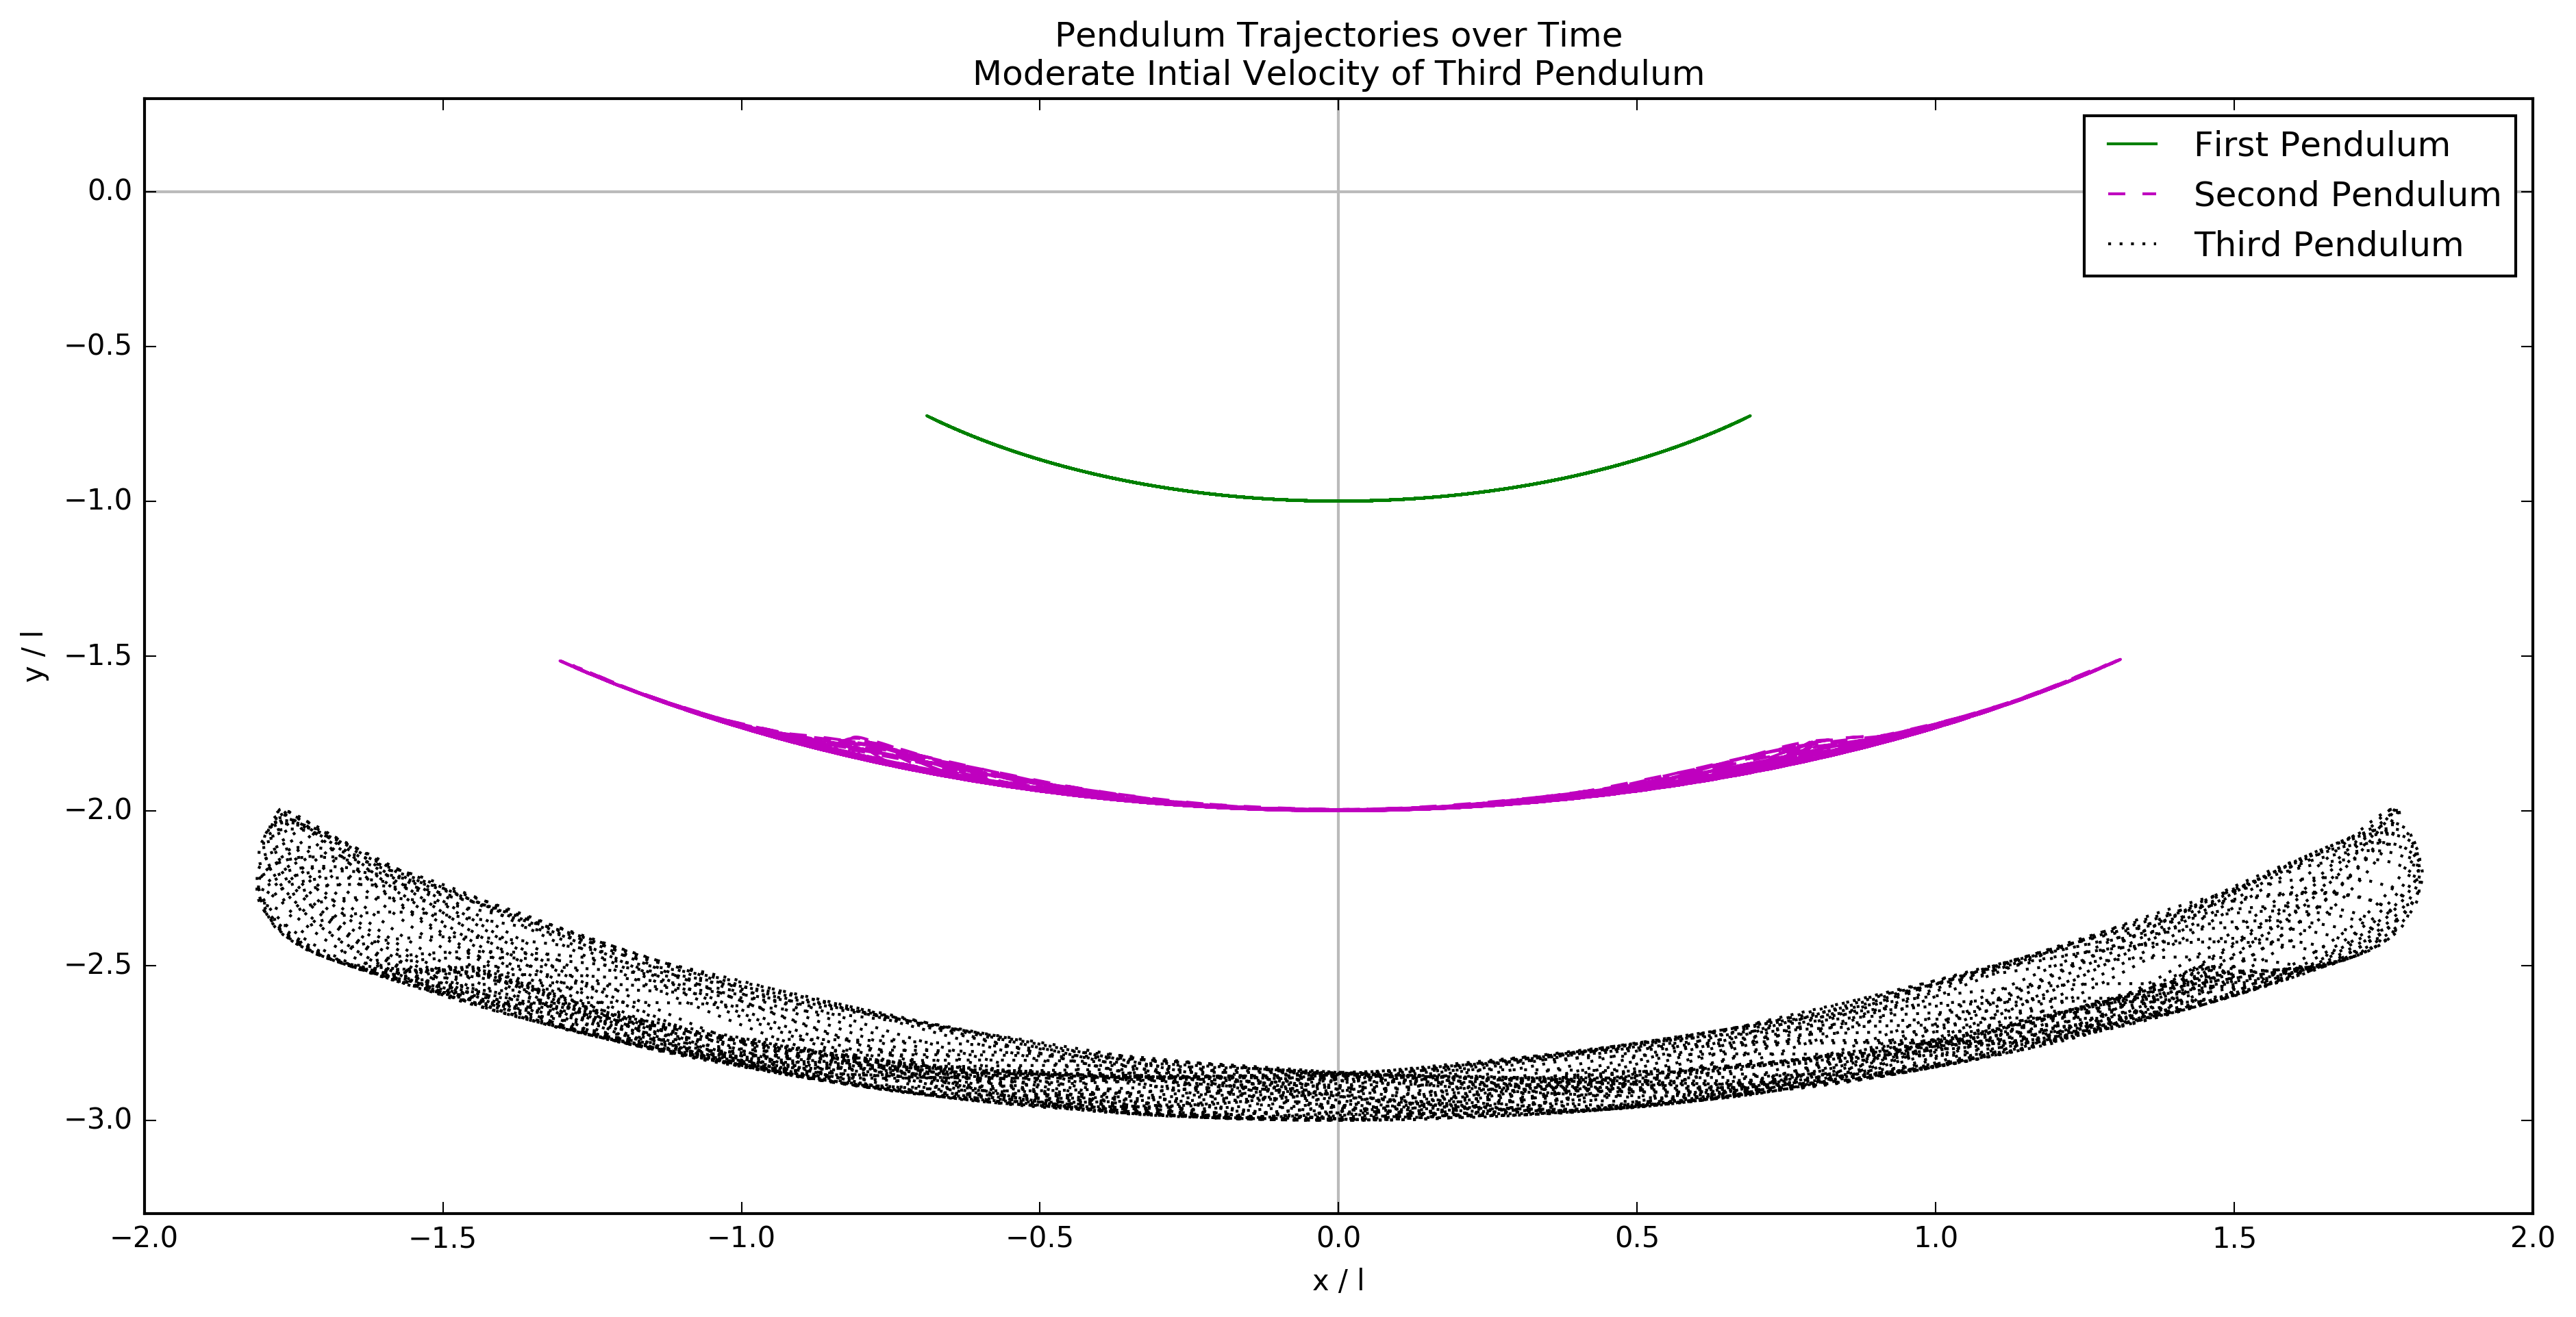
\includegraphics[width=0.5\textwidth]{moderate_velocity_trajectory}
	\caption{Mass trajectories for $\dot\phi_3(0)=\SI{7}{s^{-1}}$.}
	\label{fig:moderate_trajectories}
\end{wrapfigure}

We see that the masses are confined to a fairly narrow region of space, and 
are essentially swinging back and forth together (this is confirmed by examining
the FFT plot for the non-chaotic region (Fig. \ref{fig:fft}), where the main
frequency components for each angle are equal). 

We can also create phase space plots for the system 
(Fig. \ref{fig:moderate_phase}).
Because we have three generalized coordinates, the phase space is 
six-dimensional. We plot the angle and angular velocity of each mass on 
its own two-dimensional phase space plot, essentially looking at three 
different slices of phase space.  As a result, the phase space trajectories 
cross frequently. Notice that the phase space diagrams are symmetrical.
\begin{figure}[ht]
	\centering
	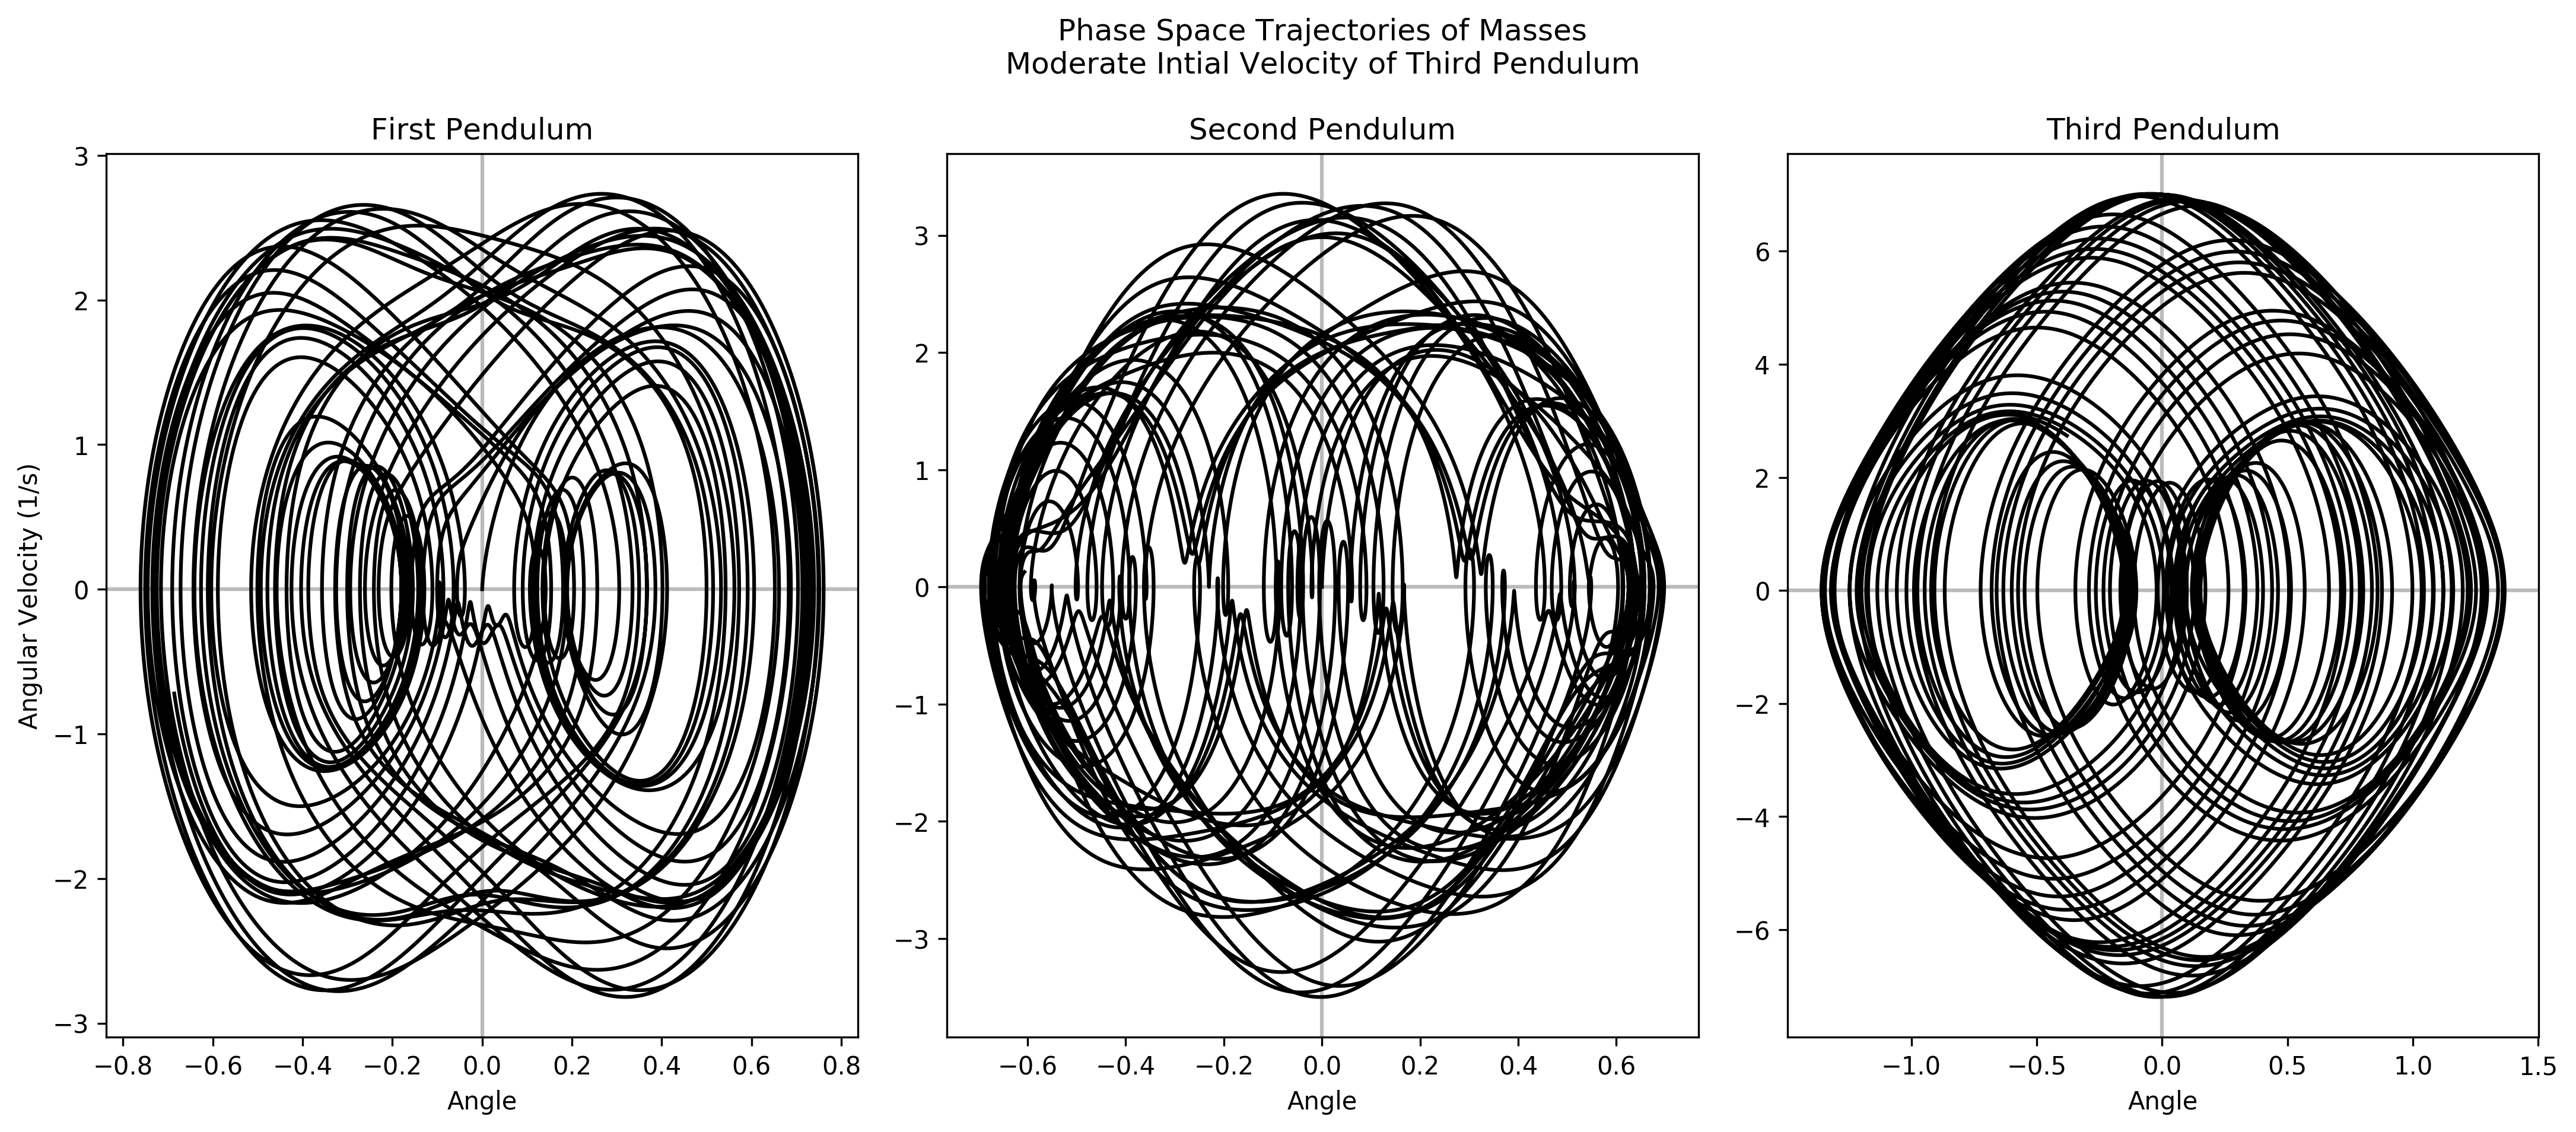
\includegraphics[width=\textwidth]{moderate_velocity_phase_space}
	\caption{Phase space slices for $\dot\phi_3(0)=\SI{7}{s^{-1}}$.}
	\label{fig:moderate_phase}
\end{figure}

\subsection{Finding Chaos}
We can use FFT contour plots to identify chaotic regions for various 
configurations of initial conditions. If instead of giving the third 
pendulum some initial velocity, we start all of the masses at rest, but 
at an equal angle from vertical, we get a much different FFT contour plot 
(Fig. \ref{fig:contour_angles}). Here we see that there is periodic behavior 
when $\phi_1(0) = \phi_2(0) = \phi_3(0) \leq 1.4$ (about $78.8\degree$). 
All initial angles past this point result in chaotic behavior. We can 
compare the periodic behavior seen in Fig. \ref{fig:moderate_trajectories} 
and Fig. \ref{fig:moderate_phase} with the chaotic behaviors seen in Fig.
\ref{fig:postcritical_trajectories} and Fig. \ref{fig:postcritical_phase}. 
The motion is no longer periodic, and the phase space trajectories no 
longer symmetrical.

\begin{figure}[ht]
	\centering
	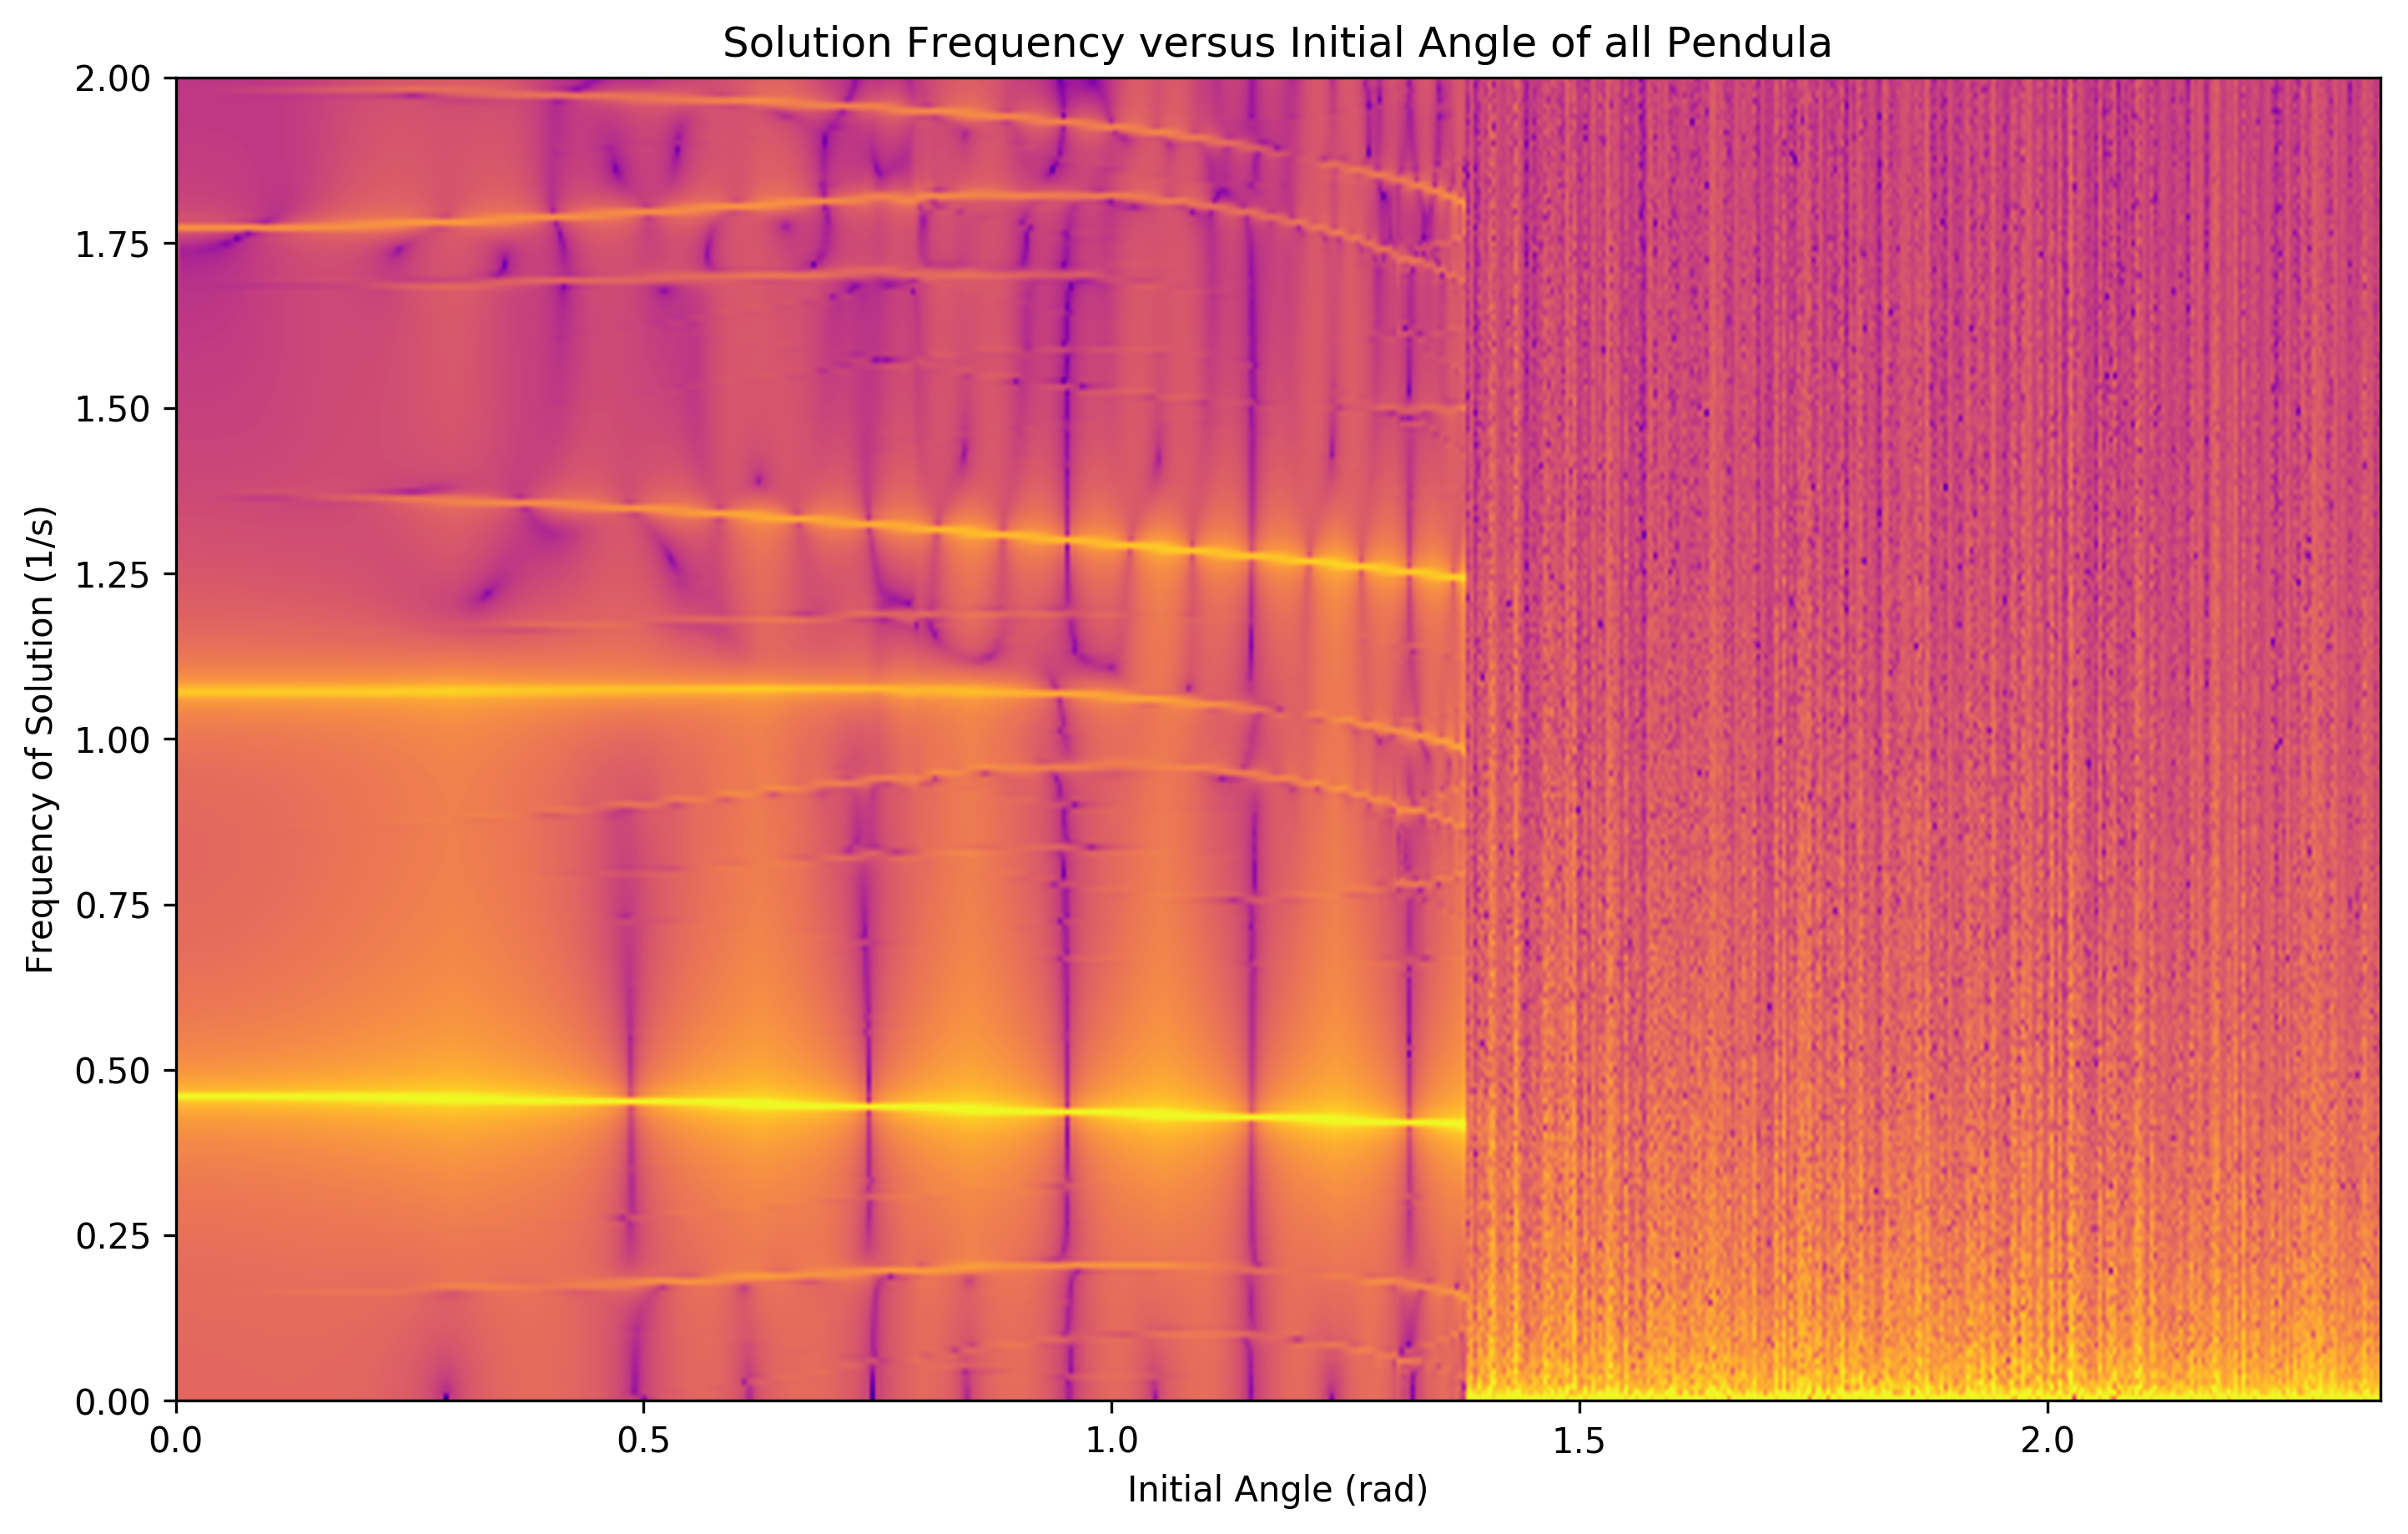
\includegraphics[width=\textwidth]{contour_angles}
	\caption{Phase space slices for $0\le\phi_i(0)\le\frac{3\pi}{4}$.}
	\label{fig:contour_angles}
\end{figure}
\begin{figure}[ht]
    \centering
    \includegraphics[width=\textwidth]{postcritical_angle_trajectory}
    \caption{Mass trajectories for $\phi_1(0)=\frac{\pi}{3}+0.04, 
    \phi_2(0)=\phi_3(0)=\frac{\pi}{3}$.}
    \label{fig:postcritical_trajectories}
\end{figure}
\begin{figure}[ht]
    \centering
    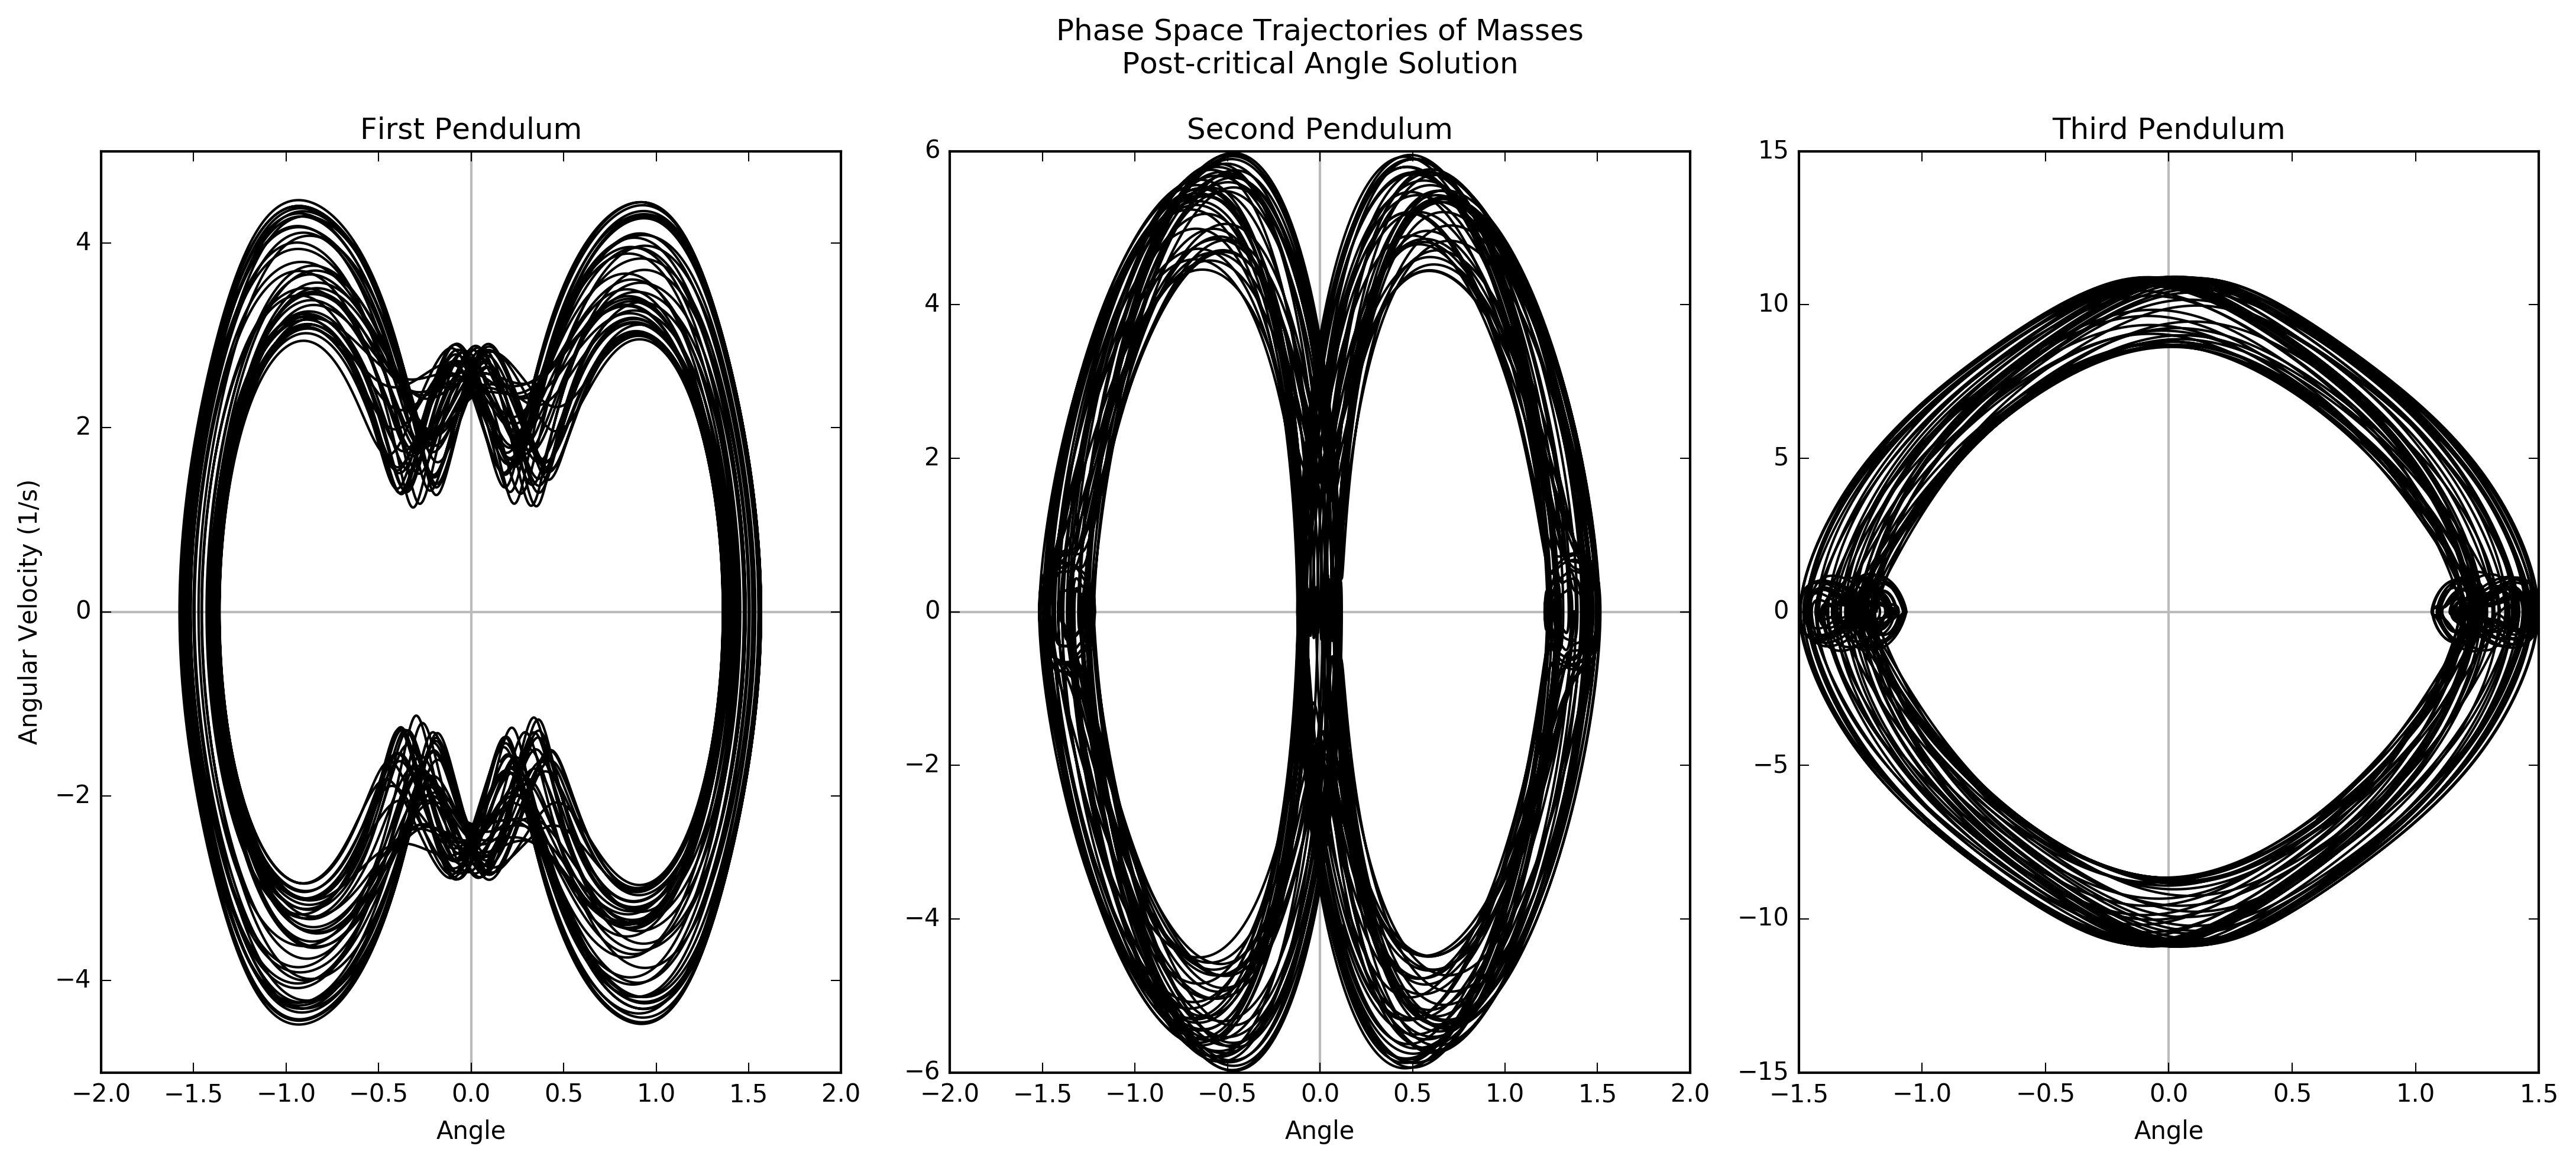
\includegraphics[width=\textwidth]{postcritical_angle_phase_space}
    \caption{Phase space slices for $\phi_1(0)=\frac{\pi}{3}+0.04, \phi_2(0) = 
    \phi_3(0)=\frac{\pi}{3}$.}
    \label{fig:postcritical_phase}
\end{figure}
        
What is special about $78.8\degree$? Examining Fig. 
\ref{fig:postcritical_trajectories}, we notice that mass $m_1$ approaches, 
but never quite crosses, horizontal.  Indeed, when the simulation is run 
again with a slightly higher initial angle, $m_1$ crosses horizontal and 
the motion becomes chaotic.

Fig. \ref{fig:max_angle} plots the maximum angle reached by $m_1$ over an
entire simulation versus the initial angles of the pendula. Below the
critical angle (in the non-chaotic region), the maximum value of $\phi_1$
increases approximately linearly as the initial angle increases. At the
critical angle the maximum value of $\phi_1$ is $90\degree$. Past this
point, the behavior is chaotic. So it seems that crossing $90\degree$ 
causes chaotic behavior.

\begin{figure}[ht]
    \centering
    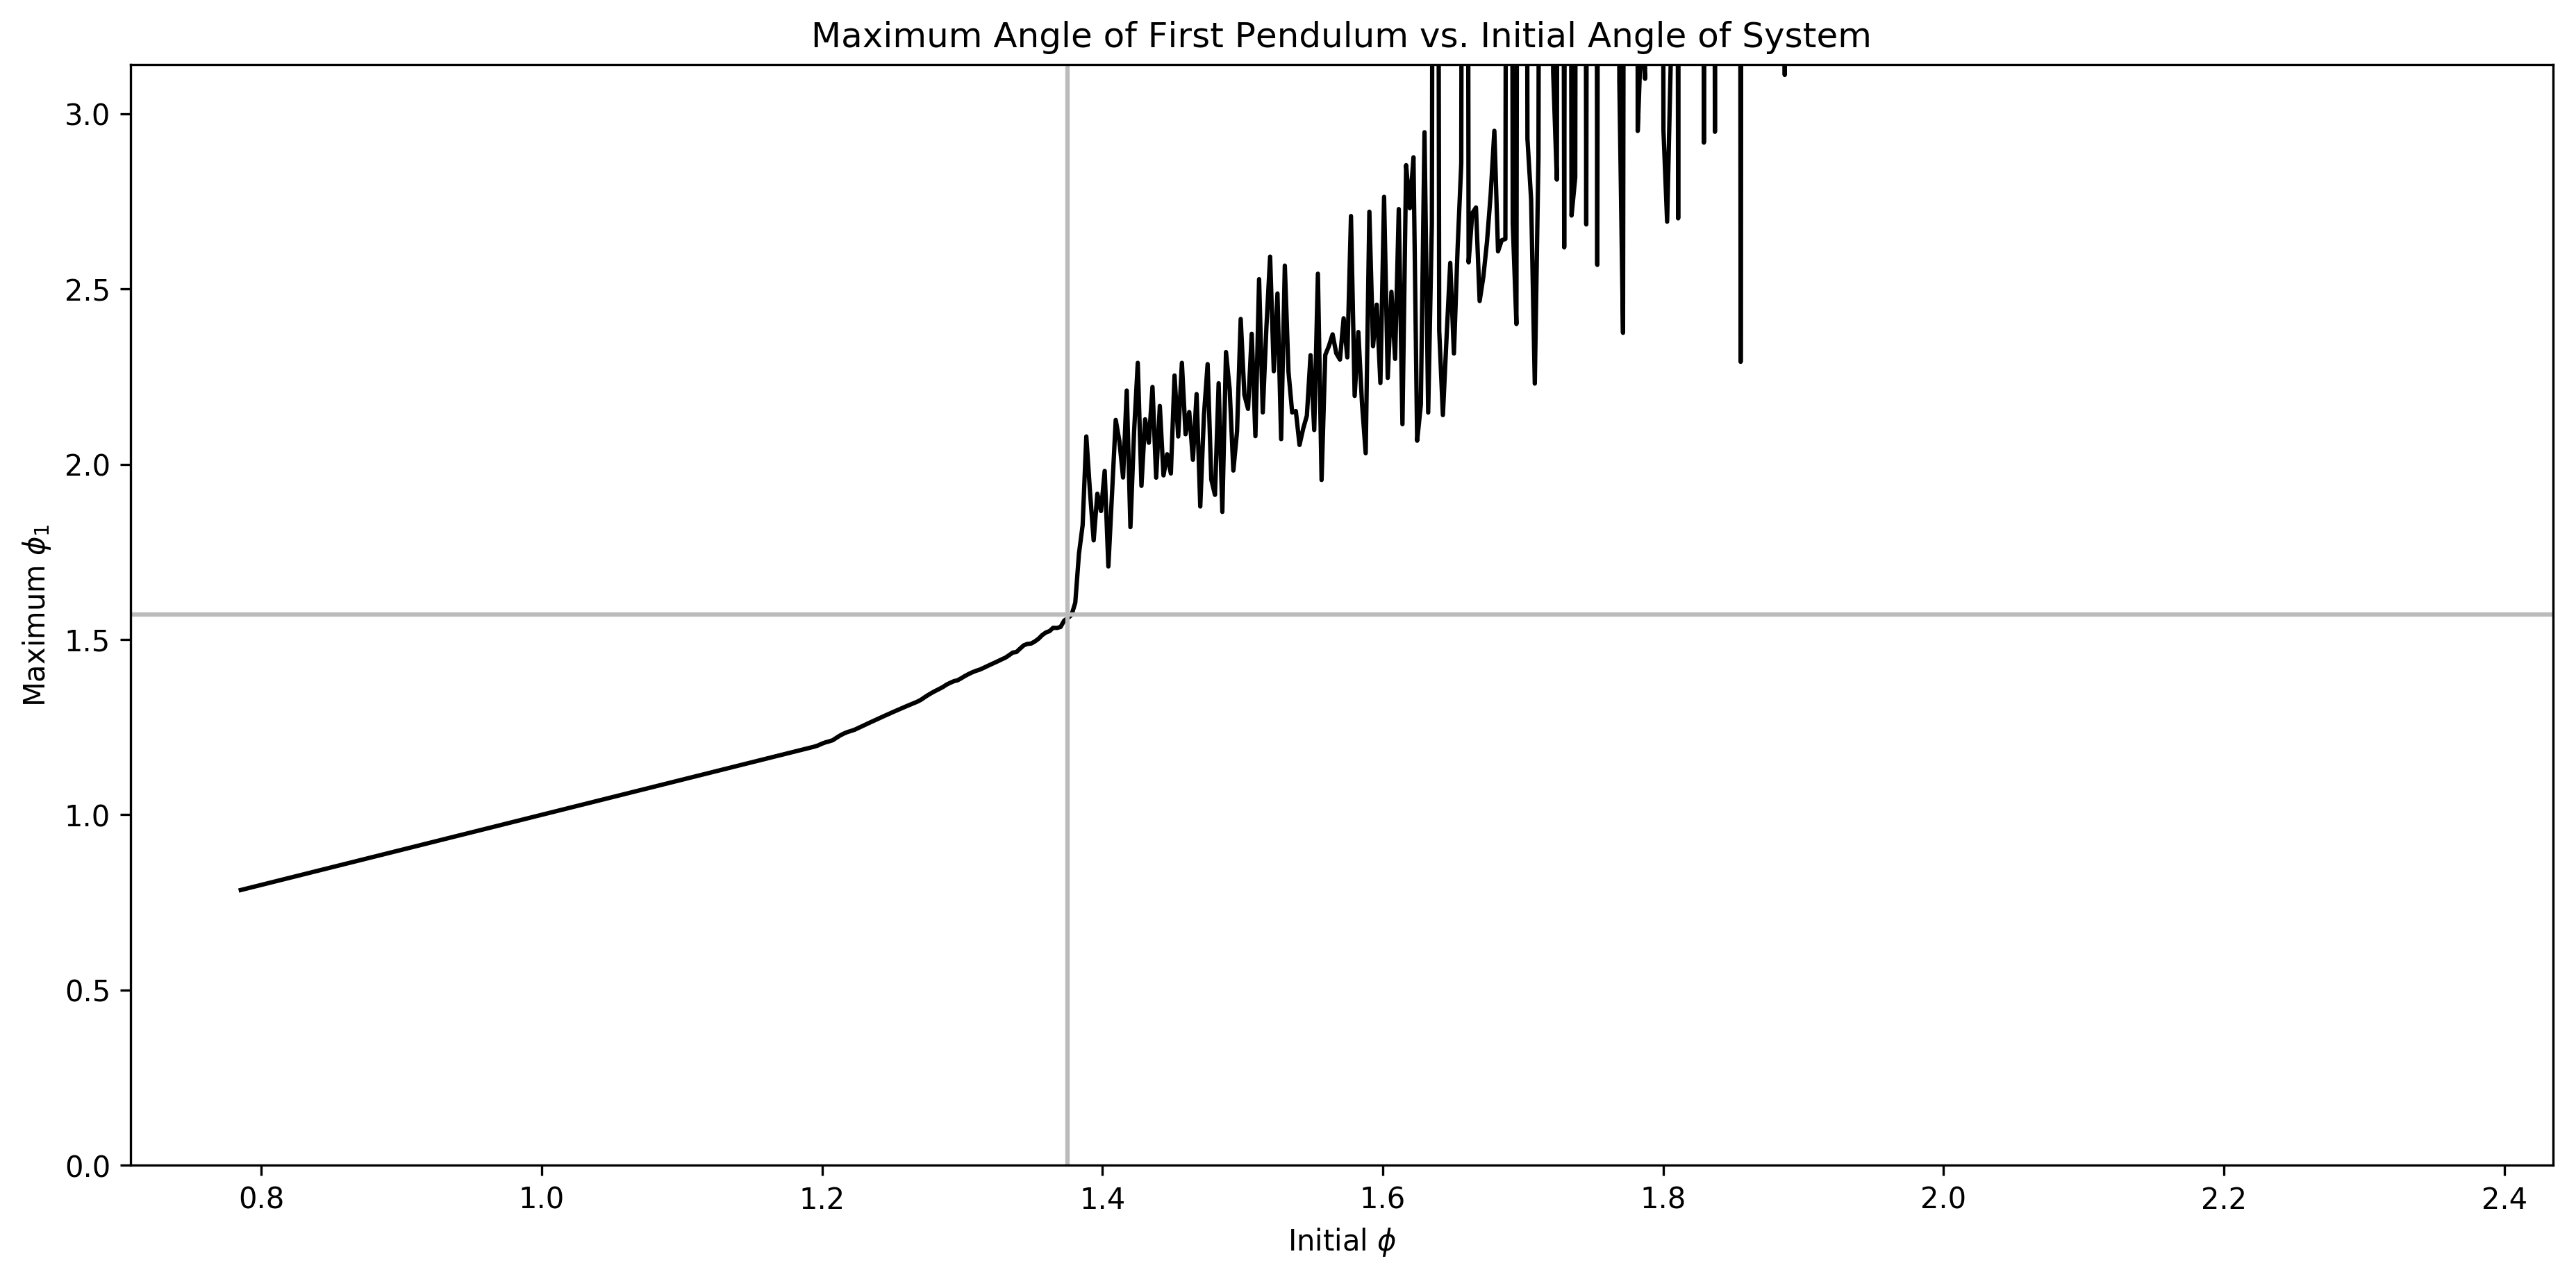
\includegraphics[width=\textwidth]{max_angle_critical}
    \caption{Plot of maximum value of $\phi_1$ versus the starting angles
    of each $\m_i$. A vertical line is drawn at the critical angle of 
    $78.8\degree$, and a horizontal line is drawn at $\phi_1=90\degree$.}
    \label{fig:max_angle}
\end{figure}


\clearpage
\begin{appendices}

\section{Equations of Motion}

\begin{wrapfigure}[13]{r}{0.25\textwidth}
	\centering
	\includegraphics[width=0.2\textwidth]{drawing.tikz}
	\caption{The triple pendulum.}
\end{wrapfigure}

We can describe the position of a given mass by its Cartesian coordinates
$(x_i, y_i)$.  The position of a given mass is the sum of its position
relative to its pivot point and the position of its pivot point:
\begin{align}
	x_1 &= l\sin\phi_1     & y_1 &= -l\cos\phi_1 \\
	x_2 &= x_1+l\sin\phi_2 & y_2 &= y_1 + -l\cos\phi_2 \\
	x_3 &= x_2+l\sin\phi_3 & y_3 &= y_2 + -l\cos\phi_3.
\end{align}
Making the appropriate substitutions, we have
\begin{align}
	x_1 &= l\sin\phi_1     \\
	y_1 &= -l\cos\phi_1 \\
	x_2 &= l(\sin\phi_1+\sin\phi_2)  \\
	y_2 &= -l(\cos\phi_1+\cos\phi_2) \\
	x_3 &= l(\sin\phi_1+\sin\phi_2+\sin\phi_3)  \\
	y_3 &= -l(\cos\phi_1+\cos\phi_2+\cos\phi_3).
\end{align}
Taking time derivatives to find velocity, we have
\begin{align}
	\dot x_1 &= l\dot\phi_1\cos\phi_1 \\
	\dot y_1 &= l\dot\phi_1\sin\phi_1 \\
	\dot x_2 &= l(\dot\phi_1\cos\phi_1+\dot\phi_2\cos\phi_2) \\
	\dot y_2 &= l(\dot\phi_1\sin\phi_1+\dot\phi_2\sin\phi_2) \\
	\dot x_3 &= l(\dot\phi_1\cos\phi_1+\dot\phi_2\cos\phi_2
		+\dot\phi_3\cos\phi_3) \\
	\dot y_3 &= l(\dot\phi_1\sin\phi_1+\dot\phi_2\sin\phi_2
		+\dot\phi_3\sin\phi_3).
\end{align}
For the kinetic energy, we will need to find $v^2={\dot x}^2{\dot y}^2$ for
each mass. 
\begin{align}
	v_1^2 &= {\dot x_1}^2+{\dot y_1}^2 \\
	&= (l\dot\phi_1\cos\phi_1)^2
		+(l\dot\phi_1\sin\phi_1)^2 \\
	&= l^2(\dot\phi_1^2\cos^2\phi_1+\dot\phi_1^2\sin^2\phi_1) \\
	&= l^2\dot\phi_1^2 \\\\
			%
	v_2^2 &= {\dot x_2}^2+{\dot y_2}^2 \\
	&= (l(\dot\phi_1\cos\phi_1+\dot\phi_2\cos\phi_2))^2
	  +(l(\dot\phi_1\sin\phi_1+\dot\phi_2\sin\phi_2))^2 \\
	&= l^2\left( \dot\phi_1^2\cos^2\phi_1 
		+ 2\dot\phi_1\dot\phi_2\cos\phi_1\cos\phi_2 
		+ \dot\phi_2^2\cos^2\phi_2 + \dot\phi_1^2\sin^2\phi_1 
		+ 2\dot\phi_1\dot\phi_2\sin\phi_1\sin\phi_2 
		+ \dot\phi_2^2\sin^2\phi_2 \right) \\
	&= l^2\left( \dot\phi_1^2\cos^2\phi_1 + \dot\phi_1^2\sin^2\phi_1
		+ \dot\phi_2^2\cos^2\phi_2 + \dot\phi_2^2\sin^2\phi_2
		+ 2\dot\phi_1\dot\phi_2(\cos\phi_1\cos\phi_2 + \sin\phi_1\sin\phi_2)
		 \right) \\
	&= l^2\left( \dot\phi_1^2 + \dot\phi_2^2
		+ 2\dot\phi_1\dot\phi_2\cos(\phi_1 - \phi_2) \right) \\\\
			%
	v_3^2 &= {\dot x_3}^2+{\dot y_3}^2 \\
	&= (l(\dot\phi_1\cos\phi_1+\dot\phi_2\cos\phi_2+\dot\phi_3\cos\phi_3))^2 
	  +(l(\dot\phi_1\sin\phi_1+\dot\phi_2\sin\phi_2+\dot\phi_3\sin\phi_3))^2 \\
	&= l^2\bigl( \dot\phi_1^2\sin^2\phi_1+\dot\phi_2^2\sin^2\phi_2
	   +\dot\phi_3^2\sin^2\phi_3 + 2\dot\phi_1\dot\phi_2\sin\phi_1\sin\phi_2
	   +2\dot\phi_1\dot\phi_3\sin\phi_1\sin\phi_3
	   +2\dot\phi_2\dot\phi_3\sin\phi_2\sin\phi_3 \\
	   &\quad +\dot\phi_1^2\cos^2\phi_1+\dot\phi_2^2\cos^2\phi_2
	   +\dot\phi_3^2\cos^2\phi_3 + 2\dot\phi_1\dot\phi_2\cos\phi_1\cos\phi_2
	   +2\dot\phi_1\dot\phi_3\cos\phi_1\cos\phi_3
	   +2\dot\phi_2\dot\phi_3\cos\phi_2\cos\phi_3
	\bigr) \\
	&= l^2\left( \dot\phi_1^2+\dot\phi_2^2 +\dot\phi_3^2 
	   +2\dot\phi_1\dot\phi_2\cos(\phi_1-\phi_2)
	   +2\dot\phi_1\dot\phi_3\cos(\phi_1-\phi_3)
	   +2\dot\phi_2\dot\phi_3\cos(\phi_2-\phi_3) \right) 
\end{align}
We can now write the kinetic and potential energy for the system by summing
up $-mgy_i$ and $\frac{1}{2}mv_i^2$ for each mass $i$:
\begin{align}
	U &= U_1 + U_2 + U_3 \\
	&= -mgl\left(3\cos\phi_1+2\cos\phi_2+\cos\phi_3 \right) \\\\
			%
	T &= T_1 + T_2 + T_3 \\
	&= \frac{1}{2}ml^2 \left( 3\dot\phi_1^2+2\dot\phi_2^2+\dot\phi_3^2
	   + 4\dot\phi_1\dot\phi_2\cos(\phi_1-\phi_2)
	   + 2\dot\phi_1\dot\phi_3\cos(\phi_1-\phi_3)
	   + 2\dot\phi_2\dot\phi_3\cos(\phi_2-\phi_3) \right) 
\end{align}
So the Lagrangian is
\begin{align}
	\L &= T - U \\
	&= mgl\left(3\cos\phi_1+2\cos\phi_2+\cos\phi_3 \right) 
	   + \frac{1}{2}ml^2 \bigl( 3\dot\phi_1^2+2\dot\phi_2^2+\dot\phi_3^2
	   + 4\dot\phi_1\dot\phi_2\cos(\phi_1-\phi_2) \\
	&\qquad\qquad + 2\dot\phi_1\dot\phi_3\cos(\phi_1-\phi_3)
	   + 2\dot\phi_2\dot\phi_3\cos(\phi_2-\phi_3) \bigr) 
\end{align}
Since our generalized coordinates are $\phi_1,\phi_2$, and $\phi_3$, we must
now take partial derivatives of the Lagrangian with respect to each $\phi_i$
and $\dot\phi_i$:
\begin{align}
	\pD{\L}{\phi_1} &= -3mgl\sin\phi_1 
		-2ml^2\dot\phi_1\dot\phi_2\sin(\phi_1-\phi_2)
		-ml^2\dot\phi_1\dot\phi_3\sin(\phi_1-\phi_3) \\
	\pD{\L}{\phi_2} &= -2mgl\sin\phi_2 
		+2ml^2\dot\phi_1\dot\phi_2\sin(\phi_1-\phi_2)
		-ml^2\dot\phi_2\dot\phi_3\sin(\phi_2-\phi_3) \\
	\pD{\L}{\phi_3} &= -mgl\sin\phi_3 
		+ml^2\dot\phi_1\dot\phi_3\sin(\phi_1-\phi_3)
		+ml^2\dot\phi_2\dot\phi_3\sin(\phi_2-\phi_3) \\\\
			%
	\pD{\L}{\dot\phi_1} &= 3ml^2\dot\phi_1 
		+ 2ml^2\dot\phi_2\cos(\phi_1-\phi_2) 
		+ ml^2\dot\phi_3\cos(\phi_1-\phi_3)  \\
	\pD{\L}{\dot\phi_2} &= 2ml^2\dot\phi_2 
		+ 2ml^2\dot\phi_1\cos(\phi_1-\phi_2) 
		+ ml^2\dot\phi_3\cos(\phi_2-\phi_3)  \\
	\pD{\L}{\dot\phi_3} &= ml^2\dot\phi_3 
		+ ml^2\dot\phi_1\cos(\phi_1-\phi_3) 
		+ ml^2\dot\phi_2\cos(\phi_2-\phi_3) 
\end{align}
Next, we find $\D{}{t}\pD{\L}{\dot\phi_i}$ for each $i$:
\begin{align}
	\D{}{t}\pD{\L}{\dot\phi_1} &= 3ml^2\ddot\phi_1 
		+ 2ml^2\ddot\phi_2\cos(\phi_1-\phi_2) 
		- 2ml^2\dot\phi_2\sin(\phi_1-\phi_2)(\dot\phi_1-\dot\phi_2) \\
		&\quad + ml^2\ddot\phi_3\cos(\phi_1-\phi_3) 
		- ml^2\dot\phi_3\sin(\phi_1-\phi_3)(\dot\phi_1-\dot\phi_3) \\\\
	\D{}{t}\pD{\L}{\dot\phi_2} &= 2ml^2\ddot\phi_2 
		+ 2ml^2\ddot\phi_1\cos(\phi_1-\phi_2) 
		- 2ml^2\dot\phi_1\sin(\phi_1-\phi_2)(\dot\phi_1-\dot\phi_2) \\
		&\quad + ml^2\ddot\phi_3\cos(\phi_2-\phi_3) 
		- ml^2\dot\phi_3\sin(\phi_2-\phi_3)(\dot\phi_2-\dot\phi_3) \\\\
	\D{}{t}\pD{\L}{\dot\phi_3} &= ml^2\ddot\phi_3 
		+ ml^2\ddot\phi_1\cos(\phi_1-\phi_3) 
		- ml^2\dot\phi_1\sin(\phi_1-\phi_3)(\dot\phi_1-\dot\phi_3) \\
		&\quad + ml^2\ddot\phi_2\cos(\phi_2-\phi_3) 
		- ml^2\dot\phi_2\sin(\phi_2-\phi_3)(\dot\phi_2-\dot\phi_3) 
\end{align}
We can then write the equations of motion for each of our generalized
coordinates, according to the Euler-Lagrange condition $\pD{\L}{\phi_i}
=\D{}{t}\pD{\L}{\dot\phi_i}$. For $\phi_1$ we have
\begin{align}
	\pD{\L}{\phi_1} &= \D{}{t}\pD{\L}{\dot\phi_1} 
\end{align}
\begin{align}
	-3mgl\sin\phi_1 -2ml^2\dot\phi_1\dot\phi_2\sin(\phi_1-\phi_2)
		-ml^2\dot\phi_1\dot\phi_3\sin(\phi_1-\phi_3)
	&= 3ml^2\ddot\phi_1 + 2ml^2\ddot\phi_2\cos(\phi_1-\phi_2) \\
	&\quad - 2ml^2\dot\phi_2\sin(\phi_1-\phi_2)(\dot\phi_1-\dot\phi_2) \\
	&\quad + ml^2\ddot\phi_3\cos(\phi_1-\phi_3) \\
	&\quad - ml^2\dot\phi_3\sin(\phi_1-\phi_3)(\dot\phi_1-\dot\phi_3) 
\end{align}
\begin{align}
	-3mgl\sin\phi_1 &= 3ml^2\ddot\phi_1 + 2ml^2\ddot\phi_2\cos(\phi_1-\phi_2)
		+ ml^2\ddot\phi_3\cos(\phi_1-\phi_3)  \\
		&\quad + 2ml^2\dot\phi_2^2\sin(\phi_1-\phi_2)
		+ ml^2\dot\phi_3^2\sin(\phi_1-\phi_3)
\end{align}
\begin{align}
	-\frac{3g}{l}\sin\phi_1 &= 3\ddot\phi_1 + 2\ddot\phi_2\cos(\phi_1-\phi_2)
		+ \ddot\phi_3\cos(\phi_1-\phi_3) + 2\dot\phi_2^2\sin(\phi_1-\phi_2)
		+ \dot\phi_3^2\sin(\phi_1-\phi_3)   \label{eq_m1}
\end{align}

For $\phi_2$ we have
\begin{align}
	\pD{\L}{\phi_2} &= \D{}{t}\pD{\L}{\dot\phi_2} 
\end{align}
\begin{align}
	-2mgl\sin\phi_2 +2ml^2\dot\phi_1\dot\phi_2\sin(\phi_1-\phi_2)
		-ml^2\dot\phi_2\dot\phi_3\sin(\phi_2-\phi_3)
	&= 2ml^2\ddot\phi_2 + 2ml^2\ddot\phi_1\cos(\phi_1-\phi_2) \\
	&\quad - 2ml^2\dot\phi_1\sin(\phi_1-\phi_2)(\dot\phi_1-\dot\phi_2) \\
	&\quad + ml^2\ddot\phi_3\cos(\phi_2-\phi_3) \\
	&\quad - ml^2\dot\phi_3\sin(\phi_2-\phi_3)(\dot\phi_2-\dot\phi_3) 
\end{align}
\begin{align}
	-2mgl\sin\phi_2 &= 2ml^2\ddot\phi_2 + 2ml^2\ddot\phi_1\cos(\phi_1-\phi_2)
		+ ml^2\ddot\phi_3\cos(\phi_2-\phi_3)  \\
		&\quad - 2ml^2\dot\phi_1^2\sin(\phi_1-\phi_2)
		+ ml^2\dot\phi_3^2\sin(\phi_2-\phi_3)
\end{align}
\begin{align}
	-\frac{2g}{l}\sin\phi_2 &= 2\ddot\phi_2 + 2\ddot\phi_1\cos(\phi_1-\phi_2)
		+ \ddot\phi_3\cos(\phi_2-\phi_3) - 2\dot\phi_1^2\sin(\phi_1-\phi_2)
		+ \dot\phi_3^2\sin(\phi_2-\phi_3)   \label{eq_m2}
\end{align}

For $\phi_3$ we have
\begin{align}
	\pD{\L}{\phi_3} &= \D{}{t}\pD{\L}{\dot\phi_3} 
\end{align}
\begin{align}
	-mgl\sin\phi_3 +ml^2\dot\phi_1\dot\phi_3\sin(\phi_1-\phi_3)
		+ml^2\dot\phi_2\dot\phi_3\sin(\phi_2-\phi_3)
	&= ml^2\ddot\phi_3 + ml^2\ddot\phi_1\cos(\phi_1-\phi_3) \\
	&\quad - ml^2\dot\phi_1\sin(\phi_1-\phi_3)(\dot\phi_1-\dot\phi_3) \\
	&\quad + ml^2\ddot\phi_2\cos(\phi_2-\phi_3) \\
	&\quad - ml^2\dot\phi_2\sin(\phi_2-\phi_3)(\dot\phi_2-\dot\phi_3) 
\end{align}
\begin{align}
	-mgl\sin\phi_3 &= ml^2\ddot\phi_3 + ml^2\ddot\phi_1\cos(\phi_1-\phi_3)
		+ ml^2\ddot\phi_2\cos(\phi_2-\phi_3)  \\
		&\quad - ml^2\dot\phi_1^2\sin(\phi_1-\phi_3)
		- ml^2\dot\phi_2^2\sin(\phi_2-\phi_3)
\end{align}
\begin{align}
	-\frac{g}{l}\sin\phi_3 &= \ddot\phi_3 + \ddot\phi_1\cos(\phi_1-\phi_3)
		+ \ddot\phi_2\cos(\phi_2-\phi_3) - \dot\phi_1^2\sin(\phi_1-\phi_3)
		- \dot\phi_2^2\sin(\phi_2-\phi_3)   \label{eq_m3}
\end{align}


Rearranging $\eqref{eq_m1}$, $\eqref{eq_m2}$, and $\eqref{eq_m3}$ by moving
the second derivatives to one side, we have
\begin{align}
	 3\ddot\phi_1 + 2\ddot\phi_2\cos(\phi_1-\phi_2) + \ddot\phi_3\cos(\phi_1-\phi_3) + 
		 &= -2\dot\phi_2^2\sin(\phi_1-\phi_2) - \dot\phi_3^2\sin(\phi_1-\phi_3)
		 -\frac{3g}{l}\sin\phi_1 \\
	2\ddot\phi_1\cos(\phi_1-\phi_2)+ 2\ddot\phi_2 + \ddot\phi_3\cos(\phi_2-\phi_3)
		&= 2\dot\phi_1^2\sin(\phi_1-\phi_2) - \dot\phi_3^2\sin(\phi_2-\phi_3)
		-\frac{2g}{l}\sin\phi_2 \\
	\ddot\phi_1\cos(\phi_1-\phi_3)+\ddot\phi_2\cos(\phi_2-\phi_3)+\ddot\phi_3
		&= + \dot\phi_1^2\sin(\phi_1-\phi_3) + \dot\phi_2^2\sin(\phi_2-\phi_3)
		-\frac{g}{l}\sin\phi_3
\end{align}
We can rewrite this system  equations as a single matrix equation:
\begingroup 
\begin{equation} 
	\renewcommand*{\arraystretch}{1.75} % more vertical space in matrix
	\resizebox{0.95\textwidth}{!}{$
	\begin{pmatrix}
		3                    & 2\cos(\phi_1-\phi_2) & \cos(\phi_1-\phi_3) \\
		2\cos(\phi_1-\phi_2) & 2                    & \cos(\phi_2-\phi_3) \\
		\cos(\phi_1-\phi_3)  & \cos(\phi_2-\phi_3)  & 1                   \\
	\end{pmatrix}
	\begin{pmatrix}
		\ddot\phi_1 \\
		\ddot\phi_2 \\
		\ddot\phi_3
	\end{pmatrix} =
	\begin{pmatrix}
		-\dot\phi_3^2\sin(\phi_1-\phi_3) -2\dot\phi_2^2\sin(\phi_1-\phi_2)
			-\frac{3g}{l}\sin\phi_1 \\
		-\dot\phi_3^2\sin(\phi_2-\phi_3) + 2\dot\phi_1^2\sin(\phi_1-\phi_2)
			-\frac{2g}{l}\sin\phi_2 \\
		\dot\phi_2^2\sin(\phi_2-\phi_3) + \dot\phi_1^2\sin(\phi_1-\phi_3)
			-\frac{g}{l}\sin\phi_3
	\end{pmatrix}
	$}
\end{equation} 
\endgroup 
We can then solve for our vector of second derivatives by multiplying on the
left by the inverse of the first matrix:
\begingroup 
\begin{equation} \renewcommand*{\arraystretch}{1.75} % more vertical space in matrix
	\resizebox{0.95\textwidth}{!}{$
	\begin{pmatrix}
		\ddot\phi_1 \\
		\ddot\phi_2 \\
		\ddot\phi_3
	\end{pmatrix} =
	\begin{pmatrix}
		3                    & 2\cos(\phi_1-\phi_2) & \cos(\phi_1-\phi_3) \\
		2\cos(\phi_1-\phi_2) & 2                    & \cos(\phi_2-\phi_3) \\
		\cos(\phi_1-\phi_3)  & \cos(\phi_2-\phi_3)  & 1                   \\
	\end{pmatrix}^{-1}
	\begin{pmatrix}
		-\dot\phi_3^2\sin(\phi_1-\phi_3) -2\dot\phi_2^2\sin(\phi_1-\phi_2)
			-\frac{3g}{l}\sin\phi_1 \\
		-\dot\phi_3^2\sin(\phi_2-\phi_3) + 2\dot\phi_1^2\sin(\phi_1-\phi_2)
			-\frac{2g}{l}\sin\phi_2 \\
		\dot\phi_2^2\sin(\phi_2-\phi_3) + \dot\phi_1^2\sin(\phi_1-\phi_3)
			-\frac{g}{l}\sin\phi_3
	\end{pmatrix}
	$} \label{mat-eqn}
\end{equation} 
\endgroup 
The matrix inverse in the above equation is very tedious to calculate. We
used a computer algebra system\footnote{SageMath, the Sage Mathematics
	Software System (Version 7.6), The Sage Developers, 2017,
	\texttt{http://www.sagemath.org}.}
to do the inverse and the matrix multiplication afterwards. The result is
\begingroup 
\begin{equation} 
	\renewcommand*{\arraystretch}{2.5} % more vertical space in matrix
	\resizebox{0.98\textwidth}{!}{$
	\begin{pmatrix}
		\ddot\phi_1 \\
		\ddot\phi_2 \\
		\ddot\phi_3
	\end{pmatrix} =
	\begin{pmatrix}
		\frac{1}{3} {\left(2 \dot\phi_2^2 \sin(\phi_1-\phi_2)-\dot\phi_3^2 \sin(\phi_1-\phi_3)-\frac{3 g \sin\left( \phi_1\right)}{l}\right)} {\left(\frac{2 {\left(\frac{{\left(2 \cos(\phi_1-\phi_2) \cos(\phi_1-\phi_3)- 3 \cos(\phi_2-\phi_3)\right)} \cos(\phi_1-\phi_2)}{2 \cos(\phi_1-\phi_2)^2- 3}-\cos(\phi_1-\phi_3)\right)}^2}{2 \cos(\phi_1-\phi_3)^2-\frac{{\left(2 \cos(\phi_1-\phi_2) \cos(\phi_1-\phi_3)- 3 \cos(\phi_2-\phi_3)\right)}^2}{2 \cos(\phi_1-\phi_2)^2- 3}- 6} + \frac{2 \cos(\phi_1-\phi_2)^2}{2 \cos(\phi_1-\phi_2)^2- 3}- 1\right)}- {\left(2 \dot\phi_1^2 \sin(\phi_1-\phi_2)-\dot\phi_3^2 \sin(\phi_2-\phi_3)-\frac{2 g \sin\left(\phi_1\right)}{l}\right)} {\left(\frac{{\left(2 \cos(\phi_1-\phi_2) \cos(\phi_1-\phi_3)- 3 \cos(\phi_2-\phi_3)\right)} {\left(\frac{{\left(2 \cos(\phi_1-\phi_2) \cos(\phi_1-\phi_3)- 3 \cos(\phi_2-\phi_3)\right)} \cos(\phi_1-\phi_2)}{2 \cos(\phi_1-\phi_2)^2- 3}-\cos(\phi_1-\phi_3)\right)}}{{\left(2 \cos(\phi_1-\phi_2)^2- 3\right)} {\left(2 \cos(\phi_1-\phi_3)^2-\frac{{\left(2 \cos(\phi_1-\phi_2) \cos(\phi_1-\phi_3)- 3 \cos(\phi_2-\phi_3)\right)}^2}{2 \cos(\phi_1-\phi_2)^2- 3}- 6\right)}} + \frac{\cos(\phi_1-\phi_2)}{2 \cos(\phi_1-\phi_2)^2- 3}\right)} + \frac{2 {\left(\dot\phi_1^2 \sin(\phi_1-\phi_3)-\dot\phi_2^2 \sin(\phi_2-\phi_3)-\frac{g \sin\left(\phi_1\right)}{l}\right)} {\left(\frac{{\left(2 \cos(\phi_1-\phi_2) \cos(\phi_1-\phi_3)- 3 \cos(\phi_2-\phi_3)\right)} \cos(\phi_1-\phi_2)}{2 \cos(\phi_1-\phi_2)^2- 3}-\cos(\phi_1-\phi_3)\right)}}{2 \cos(\phi_1-\phi_3)^2-\frac{{\left(2 \cos(\phi_1-\phi_2) \cos(\phi_1-\phi_3)- 3 \cos(\phi_2-\phi_3)\right)}^2}{2 \cos(\phi_1-\phi_2)^2- 3}- 6} \\
		-{\left(2 \dot\phi_2^2 \sin(\phi_1-\phi_2)-\dot\phi_3^2 \sin(\phi_1-\phi_3)-\frac{3 g\sin\left(\phi_1\right)}{l}\right)} {\left(\frac{{\left(2 \cos(\phi_1-\phi_2) \cos(\phi_1-\phi_3)- 3 \cos(\phi_2-\phi_3)\right)} {\left(\frac{{\left(2 \cos(\phi_1-\phi_2) \cos(\phi_1-\phi_3)- 3 \cos(\phi_2-\phi_3)\right)} \cos(\phi_1-\phi_2)}{2 \cos(\phi_1-\phi_2)^2- 3}-\cos(\phi_1-\phi_3)\right)}}{{\left(2 \cos(\phi_1-\phi_2)^2- 3\right)} {\left(2 \cos(\phi_1-\phi_3)^2-\frac{{\left(2 \cos(\phi_1-\phi_2) \cos(\phi_1-\phi_3)- 3 \cos(\phi_2-\phi_3)\right)}^2}{2 \cos(\phi_1-\phi_2)^2- 3}- 6\right)}} + \frac{\cos(\phi_1-\phi_2)}{2 \cos(\phi_1-\phi_2)^2- 3}\right)} + \frac{3}{2} {\left(2 \dot\phi_1^2 \sin(\phi_1-\phi_2)-\dot\phi_3^2 \sin(\phi_2-\phi_3)-\frac{2 g \sin\left(\phi_1\right)}{l}\right)} {\left(\frac{1}{2 \cos(\phi_1-\phi_2)^2- 3} + \frac{{\left(2 \cos(\phi_1-\phi_2) \cos(\phi_1-\phi_3)- 3 \cos(\phi_2-\phi_3)\right)}^2}{{\left(2 \cos(\phi_1-\phi_2)^2- 3\right)}^2 {\left(2 \cos(\phi_1-\phi_3)^2-\frac{{\left(2 \cos(\phi_1-\phi_2) \cos(\phi_1-\phi_3)- 3 \cos(\phi_2-\phi_3)\right)}^2}{2 \cos(\phi_1-\phi_2)^2- 3}- 6\right)}}\right)}-\frac{3 {\left(\dot\phi_1^2 \sin(\phi_1-\phi_3)-\dot\phi_2^2 \sin(\phi_2-\phi_3)-\frac{g \sin\left(\phi_1\right)}{l}\right)} {\left(2 \cos(\phi_1-\phi_2) \cos(\phi_1-\phi_3)- 3 \cos(\phi_2-\phi_3)\right)}}{{\left(2 \cos(\phi_1-\phi_2)^2- 3\right)} {\left(2 \cos(\phi_1-\phi_3)^2-\frac{{\left(2 \cos(\phi_1-\phi_2) \cos(\phi_1-\phi_3)- 3 \cos(\phi_2-\phi_3)\right)}^2}{2 \cos(\phi_1-\phi_2)^2- 3}- 6\right)}} \\
	   \frac{2 {\left(2 \dot\phi_2^2 \sin(\phi_1-\phi_2)-\dot\phi_3^2 \sin(\phi_1-\phi_3)-\frac{3 g \sin\left(\phi_1\right)}{l}\right)} {\left(\frac{{\left(2 \cos(\phi_1-\phi_2) \cos(\phi_1-\phi_3)- 3 \cos(\phi_2-\phi_3)\right)} \cos(\phi_1-\phi_2)}{2 \cos(\phi_1-\phi_2)^2- 3}-\cos(\phi_1-\phi_3)\right)}}{2 \cos(\phi_1-\phi_3)^2-\frac{{\left(2 \cos(\phi_1-\phi_2) \cos(\phi_1-\phi_3)- 3 \cos(\phi_2-\phi_3)\right)}^2}{2 \cos(\phi_1-\phi_2)^2- 3}- 6} + \frac{6 {\left(\dot\phi_1^2 \sin(\phi_1-\phi_3)-\dot\phi_2^2 \sin(\phi_2-\phi_3)-\frac{g \sin\left(\phi_1\right)}{l}\right)}}{2 \cos(\phi_1-\phi_3)^2-\frac{{\left(2 \cos(\phi_1-\phi_2) \cos(\phi_1-\phi_3)- 3 \cos(\phi_2-\phi_3)\right)}^2}{2 \cos(\phi_1-\phi_2)^2- 3}- 6}-\frac{3 {\left(2 \dot\phi_1^2 \sin(\phi_1-\phi_2)-\dot\phi_3^2 \sin(\phi_2-\phi_3)-\frac{2 g \sin\left(\phi_1\right)}{l}\right)} {\left(2 \cos(\phi_1-\phi_2) \cos(\phi_1-\phi_3)- 3 \cos(\phi_2-\phi_3)\right)}}{{\left(2 \cos(\phi_1-\phi_2)^2- 3\right)} {\left(2 \cos(\phi_1-\phi_3)^2-\frac{{\left(2 \cos(\phi_1-\phi_2) \cos(\phi_1-\phi_3)- 3 \cos(\phi_2-\phi_3)\right)}^2}{2 \cos(\phi_1-\phi_2)^2- 3}- 6\right)}}
	\end{pmatrix}
	$}\, ,\vspace{0.5em}
\end{equation} 
\endgroup 
which is far too messy to use computationally. Instead, we chose to
construct the matrices in $\eqref{mat-eqn}$ in \texttt{numpy} and
numerically calculate the inverse and multiplication. Since many of the
terms are repeated (especially the trigonometric functions of angle
differences), this has the added advantage of allowing us to precompute
these functions.

\end{appendices}

\end{document}
